% =====================================================================
%  main.tex — Housing Project prep report (Agent 4 / DESIGN_AGENT)
%  Build from build/ (4 runs):
%    lualatex -interaction=nonstopmode main.tex
%    biber main
%    lualatex -interaction=nonstopmode main.tex
%    lualatex -interaction=nonstopmode main.tex
% =====================================================================
\documentclass[12pt,a4paper,oneside]{book}
% =====================================================================
%  preamble.tex — Housing Project prep report (Agent 4 / DESIGN_AGENT)
%  Toolchain (binding, brief §4): LuaLaTeX + biber + biblatex(ieee)
%    lualatex main ; biber main ; lualatex main ; lualatex main
%  Iron rule: a problem that repeats across the document is fixed HERE,
%  never by patching chapter text. Writers: request new commands via
%  comms/inbox/to_agent4.md.
% =====================================================================

% ---------- Languages: Hebrew RTL main, English LTR ----------
\usepackage[english, bidi=basic, layout=tabular.lists]{babel}
\babelprovide[main, import]{hebrew}

% ---------- Fonts: Hebrew David, English Times New Roman ----------
\babelfont{rm}{Times New Roman}
% David has no italic: synthesize slanted shapes so \emph/\textit work (Directive 5)
\babelfont[hebrew]{rm}[Scale=1.1,
  ItalicFont=David, ItalicFeatures={FakeSlant=0.15},
  BoldItalicFont=David Bold, BoldItalicFeatures={FakeSlant=0.15}]{David}
\babelfont{sf}{Arial}
\babelfont[hebrew]{sf}{Arial}
\babelfont{tt}[Scale=0.9]{Courier New}

% ---------- Page: 2.5 cm margins + 0.5 cm binding gutter (right, RTL) ----------
\usepackage[a4paper, top=2.5cm, bottom=2.5cm, right=3cm, left=2.5cm,
            headheight=15pt]{geometry}
\usepackage{setspace}
\onehalfspacing                          % line spacing 1.5 (guide ch.11)
\setlength{\parindent}{1.5em}
\setlength{\parskip}{0.25em}
\usepackage{microtype}
\raggedbottom

% ---------- Colour palette (shared with Python charts — see chat_log) ----------
\usepackage[table]{xcolor}
\definecolor{brandNavy}{HTML}{1F3A5F}    % primary: headings, frames, series 1
\definecolor{brandSteel}{HTML}{4A6FA5}   % secondary: series 2, sub-headings
\definecolor{brandRed}{HTML}{B03A2E}     % risk / critical path / series 3
\definecolor{brandAmber}{HTML}{D68910}   % warning / milestones / series 4
\definecolor{brandGreen}{HTML}{1E8449}   % cash flow / safe / series 5
\definecolor{brandOlive}{HTML}{8C8A4B}   % "why it matters to a manager"
\definecolor{brandHead}{HTML}{DCE6F2}    % table header fill
\definecolor{brandPale}{HTML}{EAF1FB}    % light fills
% Data-chart palette (A3, colour-blind validated) — use for pgfplots/TikZ charts
\definecolor{chartBlue}{HTML}{2A78D6}    % series 1
\definecolor{chartOrange}{HTML}{EB6834}  % series 2
\definecolor{chartGreen}{HTML}{1BAF7A}   % series 3
\definecolor{chartCritical}{HTML}{C62828}% threshold / critical
\definecolor{chartInk}{HTML}{0B0B0B}
\definecolor{chartGrid}{HTML}{E4E3DF}

% ---------- BiDi / English marking (guide ch.14, Prompt B1) ----------
% \en{...}         English word / phrase / acronym / number / range / % / currency — ONE LTR unit
% \textenglish{..} alias of \en (kept for compatibility)
% \term{עברית}{English}  first use of a professional term: "עברית (English)"
% \he{...}         Hebrew inside an English environment (diagram, formula, code)
% \pct{25}         -> 25%   (LTR unit);  \deal{20/80} -> deal structure (LTR unit)
% \nis{1,500}      -> ₪1,500 (LTR unit)
% \mathhe{...}     Hebrew text inside math
\newcommand{\en}[1]{\foreignlanguage{english}{#1}}
\providecommand{\textenglish}[1]{\en{#1}}
% \enb{English} -> (English): brackets + phrase in one unbreakable box
\newcommand{\enb}[1]{\mbox{(\en{#1})}}
\newcommand{\term}[2]{#1 \enb{#2}}
\newcommand{\he}[1]{\foreignlanguage{hebrew}{#1}}
% \enp{עברית}{English}   -> עברית (English); the brackets belong to the RTL run,
%                        so they stay correct also inside an English block
\newcommand{\enp}[2]{\he{#1 \enb{#2}}}
\providecommand{\texthebrew}[1]{\he{#1}}
\newcommand{\pct}[1]{\en{#1\%}}
\newcommand{\deal}[1]{\en{#1}}                         % deal structure: \deal{20/80}
\newcommand{\nis}[1]{\en{₪#1}}
\newcommand{\mathhe}[1]{\text{\he{#1}}}
% English (LTR) environment for diagrams and code; Hebrew inside via \he{}
\newenvironment{english}{\begin{otherlanguage}{english}}{\end{otherlanguage}}

% ---------- Placeholder marker (Detector greps for \todo) ----------
\newcommand{\todo}[1]{\textcolor{brandRed}{\textbf{[להשלמה: #1]}}}

% ---------- Headings ----------
\usepackage{titlesec}
\titleformat{\chapter}[display]
  {\normalfont\bfseries\color{brandNavy}}
  {\large\color{brandSteel}פרק \thechapter}{0.3em}{\LARGE}
  [\vspace{2pt}{\color{brandSteel}\titlerule[1.2pt]}]
\titlespacing*{\chapter}{0pt}{0pt}{1.4em}
\titleformat{\section}{\normalfont\Large\bfseries\color{brandNavy}}{\thesection}{0.8em}{}
\titleformat{\subsection}{\normalfont\large\bfseries\color{brandSteel}}{\thesubsection}{0.8em}{}
\titleformat{\subsubsection}{\normalfont\normalsize\bfseries}{\thesubsubsection}{0.8em}{}
\titlespacing*{\section}{0pt}{1.6ex plus .6ex minus .2ex}{0.8ex}
\titlespacing*{\subsection}{0pt}{1.3ex plus .5ex minus .2ex}{0.5ex}
\setcounter{secnumdepth}{3}
\setcounter{tocdepth}{3}                 % TOC: chapter / section / subsection / subsubsection

% ---------- Header / footer ----------
\usepackage{fancyhdr}
\pagestyle{fancy}
\fancyhf{}
\makeatletter
\renewcommand{\chaptermark}[1]{\markboth{\if@mainmatter פרק \thechapter: \fi#1}{}}
\makeatother
\fancyhead[R]{\small\color{brandSteel}\leftmark}
\fancyfoot[C]{\small\en{\thepage}}
\renewcommand{\headrulewidth}{0.4pt}
\fancypagestyle{plain}{\fancyhf{}\fancyfoot[C]{\small\en{\thepage}}\renewcommand{\headrulewidth}{0pt}}

% ---------- Tables (first column on the right; width <= 12.4 cm) ----------
\usepackage{array, tabularx, booktabs, longtable, multirow, makecell}
\renewcommand{\arraystretch}{1.25}
\newcolumntype{R}{>{\raggedleft\arraybackslash}X}
\newcolumntype{C}{>{\centering\arraybackslash}X}
\newcolumntype{L}{>{\raggedright\arraybackslash}X}
% E = English (LTR) paragraph column, flexible width: whole cell is English
% Tested quirks: \selectlanguage in a cell adds a blank line, so raw LuaTeX
% dirs are used; with colortbl loaded (xcolor[table]) the alignment is
% mirrored, so \raggedleft here yields visually LEFT-aligned English text.
% otherlanguage* tells the bidi algorithm the text is English, so brackets at
% the edge of the cell are not mirrored (R06).
\newcolumntype{E}{>{\pardir TLT\textdir TLT\raggedleft\arraybackslash
  \begin{otherlanguage*}{english}}X<{\end{otherlanguage*}}}
\newcommand{\hd}[1]{\cellcolor{brandHead}\textbf{#1}}   % header cell
\newlength{\tabmaxwidth}\setlength{\tabmaxwidth}{12.4cm} % use: \begin{tabularx}{\tabmaxwidth}{...}

% ---------- Figures, TikZ, plots ----------
\usepackage{graphicx}
\graphicspath{{figures/}}
\usepackage{tikz}
\usetikzlibrary{positioning, arrows.meta, shapes.geometric, calc, fit, backgrounds, shadows}
\usepackage{pgfplots}
\pgfplotsset{compat=1.18}
\usepackage{amsmath, amssymb}

% ---------- Captions: figure below, table above; Hebrew names ----------
\usepackage{caption}
\captionsetup{font=small, labelfont={bf,color=brandNavy}, labelsep=colon, justification=centering}
\captionsetup[table]{position=top, skip=6pt}
\captionsetup[figure]{position=bottom, skip=6pt}
\addto\captionshebrew{%
  \renewcommand{\figurename}{איור}%
  \renewcommand{\tablename}{טבלה}%
  \renewcommand{\listfigurename}{רשימת האיורים}%
  \renewcommand{\listtablename}{רשימת הטבלאות}%
  \renewcommand{\contentsname}{תוכן העניינים}%
  \renewcommand{\bibname}{מקורות}%
  \renewcommand{\abstractname}{תקציר מנהלים}%
}

% ---------- Boxes (tcolorbox) ----------
\usepackage[most]{tcolorbox}
\tcbset{reportbox/.style={enhanced, breakable=false, arc=2mm, boxrule=0.8pt,
        left=2.5mm, right=2.5mm, top=1.5mm, bottom=1.5mm,
        before skip=8pt, after skip=8pt,
        fonttitle=\bfseries\small, halign title=flush left}}
% RTL-safe boxes: under LuaLaTeX bidi=basic a tcolorbox frame opened in RTL
% mode is mirrored off the page. Fix (tested): open the box frame in an LTR
% (english) group and switch the box content/title back to Hebrew.
% Writers simply use \begin{keyfinding}...\end{keyfinding} — no extra markup.
\tcbset{rtlsafe/.style={before upper=\selectlanguage{hebrew},
        before title=\selectlanguage{hebrew}}}
\newcommand{\NewReportBox}[4]{% #1 env name, #2 default title, #3 tcb options
  \newtcolorbox{tcb@#1}[1][#2]{reportbox, rtlsafe, title={##1}, #3}%
  \newenvironment{#1}[1][#2]%
    {\begin{otherlanguage}{english}\begin{tcb@#1}[##1]}%
    {\end{tcb@#1}\end{otherlanguage}}}
\makeatletter
% Opening of EVERY chapter: why this matters to a manager (brief §7)
\NewReportBox{managerbox}{למה זה חשוב למנהל}{colback=brandOlive!8, colframe=brandOlive}{}
% Key finding
\NewReportBox{keyfinding}{ממצא מרכזי}{colback=brandPale, colframe=brandNavy,
  borderline east={3pt}{0pt}{brandNavy}}{}
% Methodology note (data, assumptions, "בהנחה כי" / "תרחיש")
\NewReportBox{methodology}{הערה מתודולוגית}{colback=gray!6, colframe=brandSteel}{}
% Research question / hypotheses (cover + ch01 + ch06)
\NewReportBox{researchquestion}{שאלת המחקר}{colback=white, colframe=brandNavy, boxrule=1.1pt}{}
% Risk / pitfall warning
\NewReportBox{riskalert}{התראת סיכון}{colback=brandRed!5, colframe=brandRed}{}
% Aliases matching the guide's template names
\NewReportBox{keybox}{מסר מרכזי}{colback=brandAmber!6, colframe=brandAmber}{}
\NewReportBox{warnbox}{שימו לב}{colback=brandRed!5, colframe=brandRed}{}
\NewReportBox{projectbox}{בפרויקט שלנו}{colback=brandNavy!5, colframe=brandNavy}{}
\makeatother

% ---------- Code ----------
\usepackage{listings}
\lstset{basicstyle=\ttfamily\small, backgroundcolor=\color{gray!8},
        frame=single, rulecolor=\color{gray!40}, breaklines=true,
        columns=fullflexible, keepspaces=true}

% ---------- Single source of truth: report metadata ----------
\newcommand{\ResearchQuestion}{%
באיזו מידה מבצעי המימון הקבלניים (כגון \en{20/80} ו־\en{20/50/30}), הלוואות הבלון ומינוף היזמים בשוק הנדל״ן הישראלי (\en{2022–2026}) משחזרים את מנגנוני הכשל של משבר הסאב־פריים (\en{2008}) ומשבר הנדל״ן בספרד, ומהי עמידות המערכת הבנקאית והיזמית בישראל בפני גל חדלות פירעון בעת ״קיר המסירות״ של \en{2026–2027}?}
\newcommand{\ReportTitle}{מבצעי מימון קבלניים ו״קיר המסירות״}
\newcommand{\ReportSubtitle}{האם שוק הנדל״ן הישראלי משחזר את מנגנוני הכשל של \en{2008} ושל ספרד?}
\newcommand{\ReportTitleEn}{Developer Financing Promotions and the “Delivery~Wall”}
\newcommand{\ReportSubtitleEn}{Is the Israeli Housing Market Reproducing the Failure Mechanisms of 2008 and of Spain?}
\newcommand{\ReportType}{עבודת מחקר על שוק הדיור}
\newcommand{\Institution}{אוניברסיטת חיפה}
\newcommand{\CourseLine}{קורס תכנות מונחה \en{AI}, החטיבה לבינה מלאכותית, סמסטר א׳ תשפ״ז}
\newcommand{\Authors}{שקד ניניו, גיא קובלרצ׳יק}
\newcommand{\Supervisor}{ד״ר יורם סגל}
\newcommand{\ReportDate}{\en{\today}}

% ---------- Bibliography: IEEE, biber ----------
\usepackage{csquotes}
% csquotes has no 'hebrew' style -> its fallback prints a bold "?" around every
% quoted title (biblatex @online/@article titles). Map Hebrew to English quotes.
\DeclareQuoteAlias{english}{hebrew}
\usepackage[backend=biber, style=ieee, sorting=none]{biblatex}
\addbibresource{references.bib}
% D09: the ieee @online driver omits the publication date; print it after the organization.
\usepackage{xpatch}
\xpatchbibdriver{online}{\printlist{organization}}{\printlist{organization}\setunit{\addcomma\space}\printdate}{}{\GenericError{}{online date patch failed}{}{}}
% Let long URLs/DOIs break anywhere (prevents overfull lines in the reference list)
\setcounter{biburlnumpenalty}{100}
\setcounter{biburlucpenalty}{100}
\setcounter{biburllcpenalty}{100}
\AtBeginBibliography{\sloppy\emergencystretch=2em}

% List of figures/tables with its TOC entry written right after the heading, so
% the page number is correct when the list starts mid-page and runs over.
\makeatletter
\newcommand{\ListWithTocEntry}[2]{\begingroup
  \let\report@starttoc\@starttoc
  \def\@starttoc##1{\addcontentsline{toc}{chapter}{#2}\nobreak\report@starttoc{##1}}%
  #1\endgroup}
\makeatother

% ---------- Hyperlinks (always last) ----------
\usepackage[unicode, hidelinks, bookmarksnumbered]{hyperref}
\usepackage{bookmark}


\begin{document}

% ---------------- Front matter (roman numbering; cover = i, copyright = ii, both unprinted) ----------------
\frontmatter
% =====================================================================
%  frontmatter/titlepage.tex — bilingual cover (counts as page i, number
%  not printed). Edit metadata in preamble.tex only. No research question,
%  abstract or keywords here (R03).
% =====================================================================
\begin{titlepage}
\thispagestyle{empty}
% Double decorative frame (R02)
\begin{tikzpicture}[remember picture, overlay]
  \draw[brandNavy, line width=2.4pt]
    ([xshift=1.2cm,yshift=1.2cm]current page.south west) rectangle
    ([xshift=-1.2cm,yshift=-1.2cm]current page.north east);
  \draw[brandSteel, line width=0.7pt]
    ([xshift=1.45cm,yshift=1.45cm]current page.south west) rectangle
    ([xshift=-1.45cm,yshift=-1.45cm]current page.north east);
\end{tikzpicture}%
\centering
\vspace*{0.4cm}
{\Large\bfseries\color{brandNavy} \Institution\par}
\vspace{0.2cm}
{\large \CourseLine\par}
\vspace{0.3cm}
{\large \ReportType\par}

\vfill
{\color{brandSteel}\rule{0.7\textwidth}{0.8pt}\par}
\vspace{0.6cm}
{\fontsize{26}{36}\selectfont\bfseries\color{brandNavy} \ReportTitle\par}
\vspace{0.4cm}
{\leftskip=1.8cm plus 1fil\rightskip=1.8cm plus 1fil
 \Large\color{brandSteel} \ReportSubtitle\par}
\vspace{0.9cm}
{\color{brandSteel}\rule{0.25\textwidth}{0.4pt}\par}
\vspace{0.9cm}
\begin{english}
{\fontsize{20}{27}\selectfont\bfseries\color{brandNavy} \ReportTitleEn\par}
\vspace{0.4cm}
{\leftskip=1.8cm plus 1fil\rightskip=1.8cm plus 1fil
 \large\color{brandSteel} \ReportSubtitleEn\par}
\end{english}
\vspace{0.6cm}
{\color{brandSteel}\rule{0.7\textwidth}{0.8pt}\par}

\vfill
\begin{tabular}{@{}r r@{}}
\textbf{מגישים:} & \Authors \\
\textbf{מנחה:}   & \Supervisor \\
\textbf{תאריך:}  & \ReportDate \\
\end{tabular}
\vspace{1cm}
\end{titlepage}

% =====================================================================
%  frontmatter/copyright.tex — page ii (R04): copyright, affiliation,
%  attribution, AI disclosure. Counter = ii, number not printed.
% =====================================================================
\clearpage
\setcounter{page}{2}
\thispagestyle{empty}
\null\vfill
\begingroup
\setlength{\parindent}{0pt}\setlength{\parskip}{0.7em}
{\large\bfseries\color{brandNavy} \ReportTitle\par}
\ReportSubtitle\par
\begin{english}
\textbf{\ReportTitleEn}\par
\ReportSubtitleEn\par
\end{english}

{\color{brandSteel}\rule{\textwidth}{0.6pt}\par}

\textbf{זכויות יוצרים.} © \en{2026} \Authors. כל הזכויות שמורות למחברים. ציטוט קצר לצורכי לימוד ומחקר מותר בציון המקור.

\textbf{שיוך אקדמי.} \Institution, \CourseLine. מנחה: \Supervisor. \ReportType\ שהוכנה במסגרת הקורס. הדעות והמסקנות הן של המחברים ואינן מבטאות עמדה רשמית של האוניברסיטה.

\textbf{ייחוס מקורות.} הנתונים והטענות שמקורם בגורמים אחרים מצוינים בגוף הטקסט ומפורטים בפרק המקורות, והזכויות בהם שמורות לבעליהן. תוצאות המודלים הן תרחישים של המחברים, ואינן תוצאות רשמיות של גוף פיקוח או של בנק.

\sloppy \textbf{גילוי נאות: שימוש בבינה מלאכותית.} הדוח הוכן בסיוע סוכני בינה מלאכותית \enp{קלוד קוד}{Claude~Code} באיתור מקורות, בניסוח, בתכנות המודלים והתרשימים, בעימוד ובבקרה. האחריות לתוכן הסופי חלה על המחברים.\par\fussy
\endgroup
\vspace*{1cm}
\clearpage

% =====================================================================
%  frontmatter/abstract.tex — executive summary (Stage-3 editor)
%  Rules: 250–350 words; problem -> question/hypotheses -> method ->
%  key findings (with numbers) -> implication; then 5–7 keywords.
% =====================================================================
\chapter*{תקציר מנהלים}
\addcontentsline{toc}{chapter}{תקציר מנהלים}
\markboth{תקציר מנהלים}{}

בין \en{2022} ל־\en{2023} העלה בנק ישראל את הריבית מ־\pct{0.10} ל־\pct{4.75}, והיקף העסקאות בשוק הדירות ירד. במקום להוריד מחירים באופן גלוי אימצו היזמים מבצעי מימון, ובהם \deal{20/80}, \deal{20/50/30} והלוואות בלון שהריבית עליהן ממומנת בידי היזם. מבצעים אלה דוחים את מבחן יכולת ההחזר של הרוכש עד יום המסירה. בספטמבר \en{2026} עמד מלאי הדירות החדשות הלא־מכורות על \en{85,080}, ומועדי המסירה של העסקאות שנחתמו בשנים \en{2023–2025} מתרכזים ב״קיר מסירות״ בשנים \en{2026–2027}.

הדוח בוחן באיזו מידה מבנים אלה משחזרים את מנגנוני הכשל של משבר הסאב־פריים בארצות הברית ושל משבר הנדל״ן בספרד, ומהי עמידות היזמים והבנקים בישראל בעת קיר המסירות. נבחנות שלוש השערות: אשראי צל המסווה ירידת מחירים (\en{H1}), לחץ החזר של רוכשים ביום המסירה (\en{H2}), והסטת הסיכון המערכתי מהבנקים אל היזמים (\en{H3}).

הגישה משלבת סקירת ספרות נושאית, השוואה רב־פרמטרית בין שלושת המשקים, וסימולציה מבנית מכוילת שנבחרה במטריצת החלטה משוקללת. הסימולציה כוללת מודל ערך נוכחי נקי, סימולציית מונטה קרלו של יחס ההחזר, רשת מבחני קיצון לפרויקט מייצג ומודל שחיקת הון (\en{CET1}) לחמש הקבוצות הבנקאיות. עובדות מוצגות עם מקור, ותוצאות המודלים מוצגות כתרחיש.

\en{H1} נתמכת חלקית: בתרחיש, עסקת \deal{20/80} גלומה בה הנחה של \en{10.9\%–12.8\%}, אך ברמת מדד המחירים הפער מצטמצם לכ־\en{1.4\%–2.0\%}. \en{H2} נתמכת בתרחיש הבסיס: כ־\pct{36} מהרוכשים חוצים יחס החזר של \pct{40}, והתוצאה רגישה לריבית. \en{H3} אינה נתמכת לפי סף ההכרעה שנקבע מראש: בתרחיש החמור יחס כיסוי החוב של היזם יורד ל־\en{0.77}, אך ההפסד הבנקאי הוא \pct{21.3} מההון העצמי של המערכת בגרסה השמרנית (הסופרת את ירידת המחיר פעמיים) ו־\pct{14.2} בגרסה המבנית, מעל הסף של \pct{10}, הנבחן לפני מס. הקביעה שברירית: אחרי מס הגרסאות חלוקות (\pct{13.9} ו־\pct{9.2}) והתוצאה אינה מכריעה; בשיעור העברה של \en{0.5}, או בכושר ספיגה על מלוא ערך הפרויקט (הגדרת הפועלים), שתיהן נמוכות מ־\pct{10}; וכשל רוכשים לבדו אינו יוצר הפסד בנקאי. בתרחיש החמור יורדים עד ארבעה בנקים אל מתחת ליחס ההון המזערי, אך חריגה זו אינה חדלות פירעון, ובאף תרחיש שנבחן בפרמטרי הבסיס (עד \en{40\%/40\%/24}) אין בנק היורד אל מתחת ל־\pct{6.5}. ישראל דומה אפוא לספרד יותר מאשר לארצות הברית, והבנקים אינם מנותקים מהפסדי היזמים.

בשלב המימוש ייאספו נתוני מסירות, ביטולים ומשכנתאות ברמת הפרויקט, המודלים יכוילו מחדש מולם, ואומדן ההפסד הבנקאי יחודד בהתאם.

\vspace{1em}
\noindent\textbf{מילות מפתח:} מבצעי מימון קבלניים; קיר המסירות; אשראי צל; מבחני קיצון; חוק המכר; משבר הסאב־פריים; מלאי דירות לא־מכורות

\tableofcontents
\begingroup     % lists of figures and tables flow on after the TOC (page budget)
\let\clearpage\relax \let\cleardoublepage\relax
\vspace{1.5em}
\ListWithTocEntry{\listoffigures}{\listfigurename}
\vspace{1.5em}
\ListWithTocEntry{\listoftables}{\listtablename}
\endgroup
% =====================================================================
%  frontmatter/acronyms.tex — list of acronyms (first column on the right)
%  Writers: add rows here (keep alphabetical by English acronym).
% =====================================================================
\chapter*{רשימת קיצורים}
\addcontentsline{toc}{chapter}{רשימת קיצורים}
\markboth{רשימת קיצורים}{}

\begin{center}
\begin{tabularx}{\tabmaxwidth}{>{\raggedleft\arraybackslash}p{1.6cm} R E}
\toprule
\hd{קיצור} & \hd{פירוש בעברית} & \hd{Full English term} \\
\midrule
\en{ARM}  & משכנתא בריבית מתעדכנת & Adjustable-Rate Mortgage \\
\en{BIS}  & הבנק להסדרי סליקה בין־לאומיים & Bank for International Settlements \\
\en{CBS}  & הלשכה המרכזית לסטטיסטיקה (למ״ס) & Central Bureau of Statistics \\
\en{CDO}  & אגרת חוב מובטחת בחוב & Collateralized Debt Obligation \\
\en{CET1} & הון עצמי רובד \en{1} & Common Equity Tier 1 \\
\en{DSCR} & יחס כיסוי שירות החוב & Debt Service Coverage Ratio \\
\en{FCIC} & הוועדה האמריקנית לחקירת המשבר הפיננסי & Financial Crisis Inquiry Commission \\
\en{LTV}  & שיעור מימון (הלוואה לשווי) & Loan-to-Value \\
\en{MBS}  & נייר ערך מגובה משכנתאות & Mortgage-Backed Security \\
\en{NPV}  & ערך נוכחי נקי & Net Present Value \\
\en{PTI}  & יחס החזר מההכנסה & Payment-to-Income \\
\en{RACI} & מטריצת אחריות & Responsible, Accountable, Consulted, Informed \\
\en{RWA} & נכסי סיכון משוקללים & Risk-Weighted Assets \\
\en{SAREB} & חברה ספרדית לניהול נכסים בעייתיים & Spanish bad-bank (Sociedad de Gestión de Activos) \\
\en{SIV} & גוף השקעה מחוץ למאזן & Structured Investment Vehicle \\
\en{VAR}  & מודל וקטור אוטו־רגרסיבי & Vector Autoregression \\
\en{WBS}  & מבנה פירוק עבודה & Work Breakdown Structure \\
\bottomrule
\end{tabularx}
\end{center}


% ---------------- Main matter (arabic numbering) ----------------
\mainmatter
% =====================================================================
% פרק 1 — מסגרת המחקר
% Owner: Agent 1 (INTRO_HISTORY_AGENT). Numbers aligned to comms/data_summary.json
% =====================================================================
\chapter{מסגרת המחקר}
\label{ch:research-framework}

\begin{managerbox}
מבצעי המימון הקבלניים הפכו בשנים \en{2023–2025} לכלי השיווק המרכזי בשוק הדירות החדשות, והם דוחים את רגע ההכרעה הפיננסית של אלפי משקי בית אל מועד המסירה. פרק זה מגדיר את הבעיה כמותית, מציג את שאלת המחקר ואת שלוש ההשערות, ומפרט כיצד כל השערה תיבחן. זוהי המסגרת להערכת החשיפה של בנק, יזם או רגולטור ל״קיר המסירות״ של \en{2026–2027}.
\end{managerbox}

\section{רקע: ממחזור ריבית למבצעי מימון}
\label{sec:ch1-background}

מחזור העלאות הריבית של בנק ישראל בשנים \en{2022–2023} (סעיף~\ref{sec:ch3-rates}) ייקר בבת אחת את המימון של רוכשי הדירות ושל היזמים, והיקף העסקאות ירד (סעיף~\ref{sec:ch3-demand}). במקום להוריד מחירים בגלוי, אימצו יזמים רבים \term{מבצעי מימון קבלניים}{\mbox{Developer Financing Promotions}}, ובראשם מבצעי \deal{20/80} ו־\deal{20/50/30} ו\term{הלוואות בלון}{Balloon/Bullet Loans} שהריבית עליהן ממומנת בידי היזם. באוגוסט \en{2026} דווחה הטבת מימון ב־\pct{30} ממכירות הקבלנים בשוק החופשי בחמשת אזורי המעקב של משרד האוצר \cite{mof_review_2026_08,nadlancenter_2026_08_promos}.

מבנים אלה דומים למנגנונים שקדמו למשבר הסאב־פריים בארצות הברית ולמשבר הנדל״ן בספרד: תשלום התחלתי נמוך באופן מלאכותי, מינוף יזמי גבוה ומלאי גדול של דירות לא־מכורות \cite{fcic2011,akin2014}. מכאן הצורך לבחון אם ישראל משחזרת את מנגנוני הכשל של \en{2008}, או שמא הבלמים המוסדיים שלה מסיטים את הסיכון למוקד אחר. איור~\ref{fig:research-funnel} מציג את הצמצום מן הזירה העולמית אל שאלת המחקר.

\begin{figure}[!htb]
\centering
\begin{english}
\begin{tikzpicture}[font=\small, lvl/.style={draw=white, line width=1.2pt},
  txt/.style={align=center, text=white, inner sep=0pt}]
% trapezoid levels: half-widths 6.2 -> 5.4 -> 4.6 -> 3.8 -> 3.0; explicit line breaks only
\path[lvl, fill=brandNavy]  (-6.2,0)    -- (6.2,0)    -- (5.4,-1.1) -- (-5.4,-1.1) -- cycle;
\path[lvl, fill=brandSteel] (-5.4,-1.1) -- (5.4,-1.1) -- (4.6,-2.2) -- (-4.6,-2.2) -- cycle;
\path[lvl, fill=brandNavy!85!brandRed] (-4.6,-2.2) -- (4.6,-2.2) -- (3.8,-3.3) -- (-3.8,-3.3) -- cycle;
\path[lvl, fill=brandRed]   (-3.8,-3.3) -- (3.8,-3.3) -- (3.0,-4.4) -- (-3.0,-4.4) -- cycle;
\node[txt] at (0,-0.55) {\he{\textbf{מחזורי אשראי ולקחי משבר הסאב־פריים}}\\\he{ארה״ב וספרד (פרקים \ref{ch:subprime}, \ref{ch:comparative})}};
\node[txt] at (0,-1.65) {\he{\textbf{שוק הדיור בישראל, \en{2022–2026}}}\\\he{ריבית, מחירים ומלאי (פרק \ref{ch:israel})}};
\node[txt] at (0,-2.75) {\he{\textbf{מבצעי קבלנים: \en{20/80}, \en{20/50/30}}}\\\he{אשראי צל (\en{H1}; פרק \ref{ch:methodology})}};
\node[txt] at (0,-3.85) {\he{\textbf{״קיר המסירות״ \en{2026–2027}}}\\\he{חוסן בנקים ויזמים (\en{H2}, \en{H3})}};
\end{tikzpicture}
\end{english}
\caption{משפך המחקר: ממחזורי האשראי העולמיים אל ״קיר המסירות״ הישראלי}
\label{fig:research-funnel}
\end{figure}

\section{הצגת הבעיה במונחים כמותיים}
\label{sec:ch1-problem}

טבלה~\ref{tab:ch1-problem} מסכמת את הבעיה: מצב נוכחי, מצב רצוי, הפער ועלותו. ערכים שמקורם בסימולציה מסומנים כתרחיש להמחשה.

\begin{table}[!htb]
\centering
\caption{הצגת הבעיה: מצב נוכחי, מצב רצוי, פער ועלות}
\label{tab:ch1-problem}
\footnotesize
\begin{tabularx}{\tabmaxwidth}{>{\raggedleft\arraybackslash}p{2.0cm} >{\hsize=.9\hsize}R >{\hsize=1.1\hsize}R}
\toprule
\hd{ממד} & \hd{מצב נוכחי (מאומת)} & \hd{מצב רצוי / פער ועלות} \\
\midrule
מלאי לא־מכור & \en{85,080} דירות חדשות לא־מכורות (ספטמבר \en{2026}); שיא של \en{86,290} בינואר \en{2026} \cite{cbs_newdwellings_2026q3,cbs_newdwellings} & מלאי התואם את קצב הספיגה. הפער: הון יזמי קשור הנושא עלויות מימון שוטפות \\
\midrule
שקיפות מחירים & מדד מחירי הדירות ירד ב־\pct{1.8} בשנה (יולי–אוגוסט \en{2026}) \cite{toi_housing_2026_10} & מחיר מדווח השווה למחיר הכלכלי. הפער: הנחה כלכלית גלומה של \en{10.9\%–12.8\%} לעסקת \deal{20/80} (תרחיש להמחשה, פרק~\ref{ch:methodology}) \\
\midrule
יכולת ההחזר של הרוכשים & הטבת מימון ב־\pct{30} ממכירות הקבלנים בשוק החופשי (חמישה אזורים, אוגוסט \en{2026}) \cite{mof_review_2026_08,nadlancenter_2026_08_promos} & יחס החזר במסירה מתחת ל־\pct{40}. הפער: בתרחיש בסיס \pct{36} מהרוכשים מעל הסף (סימולציה, פרק~\ref{ch:delivery-wall}) \\
\midrule
חשיפת המערכת הבנקאית & כ־\pct{39} מהאשראי העסקי מופנה לבינוי ולנדל״ן (\en{2025}) \cite{boi2026_recredit} & חשיפה מגודרת. העלות: הפסדי אשראי וצורך בהון נוסף אם הסיכון יעבור מהיזמים לבנקים \\
\bottomrule
\end{tabularx}
\end{table}

\noindent במשפט אחד: מבצעי המימון מחליפים כיום ירידת מחיר גלויה בהנחה סמויה, ודוחים לשנים \en{2026–2027} את מבחן יכולת ההחזר של רוכשים שמספרם הכולל לא פורסם (סעיף~\ref{sec:ch3-tam}). טרם ידוע אם הסיכון ייספג במאזני היזמים או יעבור אל המערכת הבנקאית.

\section{המסגרת התאורטית}
\label{sec:ch1-theory}

\paragraph{השערת חוסר היציבות של מינסקי.}\label{subsec:ch1-minsky}
\sloppy תקופות ממושכות של יציבות מולידות את חוסר היציבות הבא, לפי \term{השערת חוסר היציבות הפיננסית}{Financial Instability Hypothesis} \cite{minsky1986,minsky1992}. ב\term{מימון גידור}{Hedge Finance} התזרים מכסה קרן וריבית; ב\term{מימון ספקולטיבי}{Speculative Finance} הוא מכסה רק את הריבית; וב\term{מימון פונזי}{Ponzi Finance} הלווה תלוי בעליית ערך הנכס. ככל שמשקל שני האחרונים גדל, המערכת שבירה יותר, עד ל״רגע מינסקי״ \enb{Minsky Moment}. רוכש במבצע \deal{20/80} המסתמך על משכנתא עתידית בתנאים לא ידועים נמצא במבנה ספקולטיבי ואף פונזי, וכך גם יזם הממנן את ריבית הבלון מאשראי ותלוי במכירת המלאי.\par\fussy

\paragraph{מידע אסימטרי וסיכון מוסרי.}\label{subsec:ch1-asymmetric}\label{subsec:ch1-moral-hazard}
כאשר צד אחד אינו יכול להבחין באיכות הנכס או הלווה, המחיר משקף איכות ממוצעת, והמלווים נוטים לקצוב אשראי — \term{ברירה שלילית}{Adverse Selection} \cite{akerlof1970,stiglitz1981}. \term{סיכון מוסרי}{Moral Hazard} נוצר כאשר צד המוגן מהשלכות התנהגותו נוטל סיכון מוגבר \cite{holmstrom1979}. במבצעי המימון פועלים שני המנגנונים: שווי ההטבה אינו נכלל במחיר המדווח, ומבחן המשכנתא נדחה למסירה. הקצאת הסיכון בין הצדדים היא לב \en{H3}.

\paragraph{בנקאות צל ואשראי צל.}\label{subsec:ch1-shadow}
\term{בנקאות צל}{Shadow Banking} היא תיווך אשראי מחוץ למערכת המפוקחת או בדרכים העוקפות את מגבלותיה \cite{pozsar2010,gorton2012}. \term{אשראי צל}{Shadow Credit} מוגדר בעבודה זו כהסדר שמגדיל בפועל את מינוף משק הבית או היזם, אך אינו נרשם ככזה במסגרת הכללים. מבצעי \deal{20/80} עונים להגדרה: הרוכש מתחייב לרכישה מלאה, ומבחני \en{LTV/PTI} נדחים.


\section{שאלת המחקר והשערותיו}
\label{sec:ch1-rq}

\begin{researchquestion}
\ResearchQuestion
\end{researchquestion}

\noindent השאלה מתפרקת לשלוש שאלות משנה: \textbf{מנגנון} — האם המבצעים פועלים כאשראי צל המסווה ירידת מחירים ריאלית (\en{H1}); \textbf{חשיפת משקי הבית} — מה יעלה בגורלם של רוכשים בתשלומים נדחים בעת המסירה (\en{H2}); ו\textbf{מיקום הסיכון המערכתי} — במאזני הבנקים, כבארה״ב ובספרד, או במאזני היזמים ובמלאי (\en{H3}).

\label{sec:ch1-hypotheses}ניסוח ההשערות שלהלן מחייב, והוא חוזר מילה במילה בפרק~\ref{ch:delivery-wall}, שבו הן נבחנות.

\begin{researchquestion}[השערות המחקר]
\textbf{\en{H1} — אשראי צל וקשיחות מחירים מלאכותית:} מבצעי המימון הקבלניים (\deal{20/80}, \deal{20/50/30}) והלוואות הבלון תפקדו כאשראי צל \enb{Shadow Credit} שעקף את מגבלות שיעור המימון (\en{LTV}) ויחס ההחזר מההכנסה (\en{PTI}) של בנק ישראל, ויצרו קשיחות מלאכותית של מחירי המחירון, תוך הסוואת ירידה ריאלית במחיר הכלכלי של הדירה במונחי ערך נוכחי נקי (\en{NPV}).

\medskip
\textbf{\en{H2} — לחץ החזר בעת ״קיר המסירות״:} רמת ריבית המשכנתאות הגבוהה בתקופת ״קיר המסירות״ (\en{2026–2027}) תדחוף שיעור מהותי מרוכשי הדירות בתשלומים נדחים אל מעבר לסף יחס ההחזר של \pct{40} מההכנסה (\en{PTI}), שמעליו חל משקל סיכון מוגבר, ותוביל למצוקת מימון מחדש \enb{Refinancing Distress} ולביטולי עסקאות פוטנציאליים.

\medskip
\textbf{\en{H3} — הסטת הסיכון המערכתי ליזמים:} בשל הבלמים המוסדיים — חוק המכר (דירות), מנגנון הליווי הבנקאי הסגור, מגבלות \en{LTV/PTI} נוקשות והלוואות בחבות אישית מלאה \enb{Full Recourse} — הסיכון המערכתי בישראל מתרכז במאזני היזמים ובמלאי הדירות הלא־מכורות (למעלה מ־\en{85,000} יחידות) ולא בחדלות פירעון של הבנקים, כפי שאירע בארה״ב ובספרד ב־\en{2008}.
\end{researchquestion}

\section{היקף, הנחות יסוד ודרישות}
\label{sec:ch1-scope}

\paragraph{בתוך ההיקף.} שוק הדירות החדשות בישראל בשנים \en{2022–2026}; מבצעי \deal{20/80}, \deal{20/50/30} והלוואות בלון במימון היזם; רוכשים פרטיים; יזמים בליווי בנקאי סגור; חמש הקבוצות הבנקאיות הגדולות. מקרי ההשוואה: ארה״ב (\en{2004–2009}) וספרד (\en{2004–2013}). \textbf{מחוץ להיקף:} שכירות, דיור ציבורי ו״מחיר למשתכן״, נדל״ן מסחרי והשפעות מאקרו מעבר לערוץ הריבית.

\paragraph{הנחות יסוד.} (\en{1}) נתוני בנק ישראל, הלמ״ס ומשרד האוצר מהימנים, בכפוף לכך שספירת המלאי של הלמ״ס כוללת גם דירות שבנייתן טרם החלה; (\en{2}) מחיר העסקה המדווח הוא מחיר המחירון, ללא שווי ההטבה המימונית; (\en{3}) פרמטרים שאינם נצפים מכוילים ומוצגים כתרחיש (פרק~\ref{ch:methodology}); (\en{4}) תנאי הרגולציה הם אלה שבתוקף בנובמבר \en{2026}, ובהם הוראת השעה שתוקפה עד \en{31.12.2026} \cite{boi_circular2816}.

\paragraph{דרישות ושיטת אימות.}\label{sec:ch1-requirements} כל השערה מתורגמת לדרישה מדידה עם ערך יעד ושיטת אימות (טבלה~\ref{tab:ch1-requirements}). ספי ההכרעה נקבעו לפני הרצת המודלים, כדי למנוע התאמה בדיעבד.

\begin{table}[!htb]
\centering
\caption{דרישות המחקר: מזהה, דרישה, ערך יעד ושיטת אימות}
\label{tab:ch1-requirements}
\footnotesize
\begin{tabularx}{\tabmaxwidth}{>{\raggedleft\arraybackslash}p{1.95cm} >{\hsize=.9\hsize}R >{\hsize=1.15\hsize}R >{\hsize=.95\hsize}R}
\toprule
\hd{מזהה} & \hd{דרישה} & \hd{ערך יעד / סף הכרעה} & \hd{שיטת אימות} \\
\midrule
\mbox{\en{REQ-H1-01}} & אומדן ההנחה הכלכלית הגלומה בעסקאות \deal{20/80} ו־\deal{20/50/30} & \en{H1} נתמכת אם ההנחה עולה על \pct{5} בכל שיעורי ההיוון \en{5\%–6\%} & מודל \en{NPV}, פרק~\ref{ch:methodology} \\
\midrule
\mbox{\en{REQ-H1-02}} & השוואת מדד המחירים הרשמי למדד מתוקן \en{NPV} & סדרה חודשית \en{2021–2026}; פער חיובי מתמשך & מדד מתוקן מול נתוני הלמ״ס \\
\midrule
\mbox{\en{REQ-H2-01}} & התפלגות יחס ההחזר במסירה בשלושה תרחישי ריבית & \en{H2} נתמכת אם בתרחיש הבסיס \pct{20} או יותר מהרוכשים מעל \pct{40} & סימולציית מונטה קרלו, \mbox{\en{N = 10,000}}, פרק~\ref{ch:delivery-wall} \\
\midrule
\mbox{\en{REQ-H3-01}} & מבחן קיצון לפרויקט מייצג: ירידת מחירים \en{0\%–20\%} ועיכוב \en{0–24} חודשים & \en{H3} נתמכת אם בתרחיש החמור יחס הכיסוי של היזם יורד אל מתחת ל־\en{1} \enb{DSCR < 1}, בעוד ההפסד הבנקאי המוערך נמוך מ־\pct{10} מההון העצמי של המערכת & רשת \en{81} תאים ואומדן הפסד, פרק~\ref{ch:delivery-wall} \\
\midrule
\mbox{\en{REQ-CMP-01}} & השוואה רב־ממדית ארה״ב / ספרד / ישראל & \en{8} פרמטרים לפחות, כל אחד עם מקור & טבלת השוואה, פרק~\ref{ch:comparative} \\
\midrule
\mbox{\en{REQ-DAT-01}} & אמינות הנתונים & \pct{100} מהערכים העובדתיים עם מקור מאומת & הצלבה מול \en{data\_summary.json} \\
\bottomrule
\end{tabularx}
\end{table}

\paragraph{מבנה הדוח.}\label{sec:ch1-structure} מבנה הדוח עוקב אחר המשפך שבאיור~\ref{fig:research-funnel}; פרק~\ref{ch:delivery-wall} מכריע בהשערות, ופרק~\ref{ch:risks-gantt} מציג את תוכנית העבודה והסיכום. הפרק הבא פותח במשבר \en{2008} עצמו ובמה שהספרות למדה עליו.

% =====================================================================
% פרק 2 — מבוא היסטורי א': משבר הסאב־פריים בארה"ב ומשבר הנדל"ן בספרד
% Owner: Agent 1. Thematic, critical literature review (guide ch.5)
% =====================================================================
\chapter{מבוא היסטורי א': משבר הסאב־פריים בארצות הברית ומשבר הנדל״ן בספרד}
\label{ch:subprime}

\begin{managerbox}
משברי \en{2008} בארה״ב ובספרד הם שני ״תסריטים״ שונים של כשל בשוק הדיור. בארה״ב הסיכון עבר מהלווים אל המערכת הפיננסית דרך איגוח ובנקאות צל. בספרד הוא הצטבר במאזני היזמים ובקופות החיסכון שמימנו אותם. מי שמנהל חשיפה לנדל״ן צריך לדעת איזה משני התסריטים קרוב יותר למצב בישראל, ופרק זה מספק את אבני הבוחן לכך.
\end{managerbox}

משבר הסאב־פריים (\en{Subprime}) של \en{2007–2009} החל כבעיית אשראי בפלח מצומצם של שוק המשכנתאות האמריקאי, והתגלגל למשבר נזילות ופירעון עולמי \cite{fcic2011,brunnermeier2009}. במקביל קרס בספרד שוק נדל״ן שנשען על תנופת בנייה ועל אשראי יזמי \cite{akin2014,bde2017}. הסקירה מאורגנת בשישה נושאים: הסכמות, מחלוקות ורלוונטיות לישראל.

\section{נושא \en{1}: היצע אשראי מול יסודות כלכליים}
\label{sec:ch2-credit}

האם עליית המחירים בארה״ב בשנים \en{1997–2006} נבעה מיסודות כלכליים או מהיצע האשראי? ריבית של \pct{1} וביקוש עולמי לנכסים ״בטוחים״ יצרו ״רעב לתשואה״ \enb{Search for Yield} \cite{brunnermeier2009}. מיאן וסופי \cite{mian2009} מצאו שאשראי המשכנתאות התרחב מהר ביותר דווקא במיקודים שבהם שיעור הלווים בדירוג נמוך היה גבוה וצמיחת ההכנסות חלשה; מכאן שהיצע האשראי, ולא היסודות, הניע את הבועה. בהמשך הראו שהפגיעה בעושר משקי הבית הממונפים הפכה את משבר הדיור למיתון הגדול \cite{mian2014}.

\paragraph{מחלוקת.} אדלינו, שואר וסברינו \cite{adelino2016} מראים שחלק גדול מהגידול באשראי ומהכשלים התרכז דווקא במעמד הביניים ובלווים בדירוג סביר. אם הסיכון אינו מוגבל ללווים ״חלשים״, גם רוכשים בהכנסה ממוצעת במבצעי \deal{20/80} עלולים להיפגע (\en{H2}).

\section{נושא \en{2}: מוצרים הדוחים את מבחן היכולת}
\label{sec:ch2-teaser}

בלב המשבר האמריקאי עמדו מוצרי משכנתא שבהם התשלום ההתחלתי היה נמוך באופן מלאכותי \cite{fcic2011}: משכנתאות טיזר מסוג \en{2/28} או \en{3/27} (\en{Teaser}, \en{ARM}), שבהן הריבית המוזלת ״התאפסה״ (\en{Reset}) לאחר שנתיים־שלוש; הלוואות \en{Interest-Only} ו־\en{Option ARM}; והלוואות \en{Low-Doc/No-Doc} ללא הוכחת הכנסה. המשותף לכולן הוא \textbf{דחיית מבחן היכולת}, כלומר מעבר ממימון גידור למימון ספקולטיבי ופונזי \cite{minsky1992}.

איור~\ref{fig:payment-shock} ממחיש את ״זעזוע התשלום״ בפרמטרים מכוילים. בתרחיש להמחשה, הלוואה של \en{\$200,000} שעברה מריבית של \pct{8} ל־\pct{11} העלתה את ההחזר החודשי ב־\pct{29} ואת יחס ההחזר מ־\pct{40} ל־\pct{51.5}. בעסקאות \deal{20/80} ו־\deal{20/50/30} הקפיצה ביום המסירה חדה יותר: מאפס, או מ־\pct{20.5} בתשלום ריבית בלבד, ל־\pct{36} מההכנסה.

\begin{figure}[!htb]
\centering
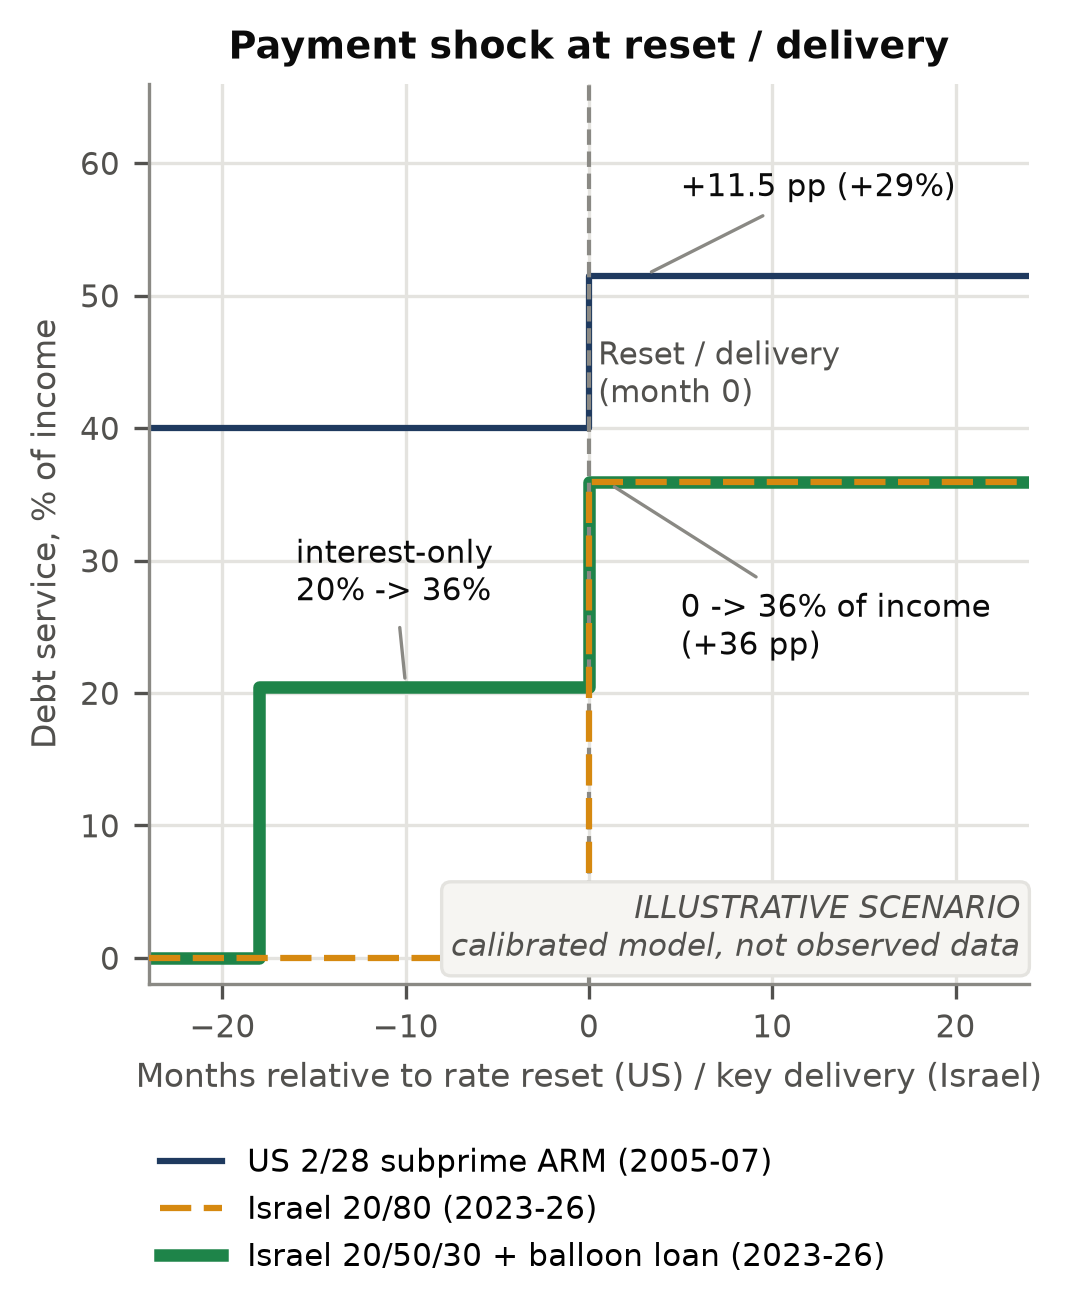
\includegraphics[width=0.62\textwidth]{figures/fig1_payment_shock_2080_vs_teaser.png}
\caption[זעזוע התשלום בנקודת האיפוס: טיזר \en{2/28} מול \en{20/80} ו־\en{20/50/30}]{זעזוע התשלום בנקודת האיפוס: משכנתת טיזר \en{2/28} בארה״ב (\en{2005–2007}) לעומת עסקאות \en{20/80} ו־\en{20/50/30} בישראל, כשיעור מהכנסת משק הבית. תרחיש להמחשה בפרמטרים מכוילים (פרק~\ref{ch:methodology})}
\label{fig:payment-shock}
\end{figure}

\section{נושא \en{3}: איגוח, דירוג וסיכון מוסרי}
\label{sec:ch2-securitization}

\sloppy מבנה התמריצים השתנה במעבר ממודל ״הפקה לשם החזקה״ \enb{Originate-to-Hold} למודל ״הפקה לשם הפצה״ \enb{Originate-to-Distribute}. מלווים, חלקם ללא פיקוח בנקאי, מכרו הלוואות לבנקי השקעות, שאיגדו אותן ל\term{ניירות ערך מגובי משכנתאות}{MBS} ואיגדו מחדש את שכבות הביניים ל\term{אגרות חוב מובטחות בחוב}{CDO}. קיז ושותפיו \cite{keys2010} מצאו שהאיגוח הוביל לסינון רשלני יותר של לווים, כתחזית תאוריית הסיכון המוסרי, ו־\pct{83} מניירות הערך שדירגה \en{Moody's} בדירוג \en{AAA} בשנת \en{2006} הורדו לבסוף בדירוגם \cite{fcic2011}. \textbf{רלוונטיות לישראל:} בישראל חקיקת האיגוח טרם הושלמה \cite{boi_survey2025,hapoalim_q3_2026}, ונראה שערוץ ההעברה המרכזי של המשבר האמריקאי אינו קיים בהיקף דומה (\en{H3}). מנגד, ההיגיון של ״מוכר שאינו נושא בסיכון״ חוזר בצורה אחרת: היזם מקבל תמורה מוקדמת, ומבחן היכולת של הרוכש נדחה.\par\fussy

\section{נושא \en{4}: בנקאות צל וריצה על הנזילות}
\label{sec:ch2-shadow}

חלק ניכר מהנכסים המאוגחים הוחזק בגופים מחוץ למאזן הבנקים (\en{SIVs}, \en{Conduits}), שמומנו בנייר ערך מסחרי קצר מועד ובהסכמי רכש חוזר (\en{Repo}). פוזסר ושותפיו \cite{pozsar2010} מעריכים שערב המשבר עלו התחייבויות מערכת הצל האמריקאית על אלה של המערכת הבנקאית המסורתית. גורטון ומטריק \cite{gorton2012} מתארים כיצד העלאת שיעורי הביטחון (\en{Haircuts}) בשוק הריפו יצרה ״ריצה״ מודרנית. \textbf{רלוונטיות לישראל:} אשראי חוץ־בנקאי ליזמים ומימון ריבית ישיר בידי היזם הם המקבילה הישראלית ל״צל״: ערוצים שהפיקוח על הבנקים אינו מגביל ישירות (\en{H1}).

\section{נושא \en{5}: עיקולים, חבות אישית והלולאה ההרסנית}
\label{sec:ch2-foreclosures}

העלאת הריבית בארה״ב מ־\pct{1} ל־\pct{5.25} (\en{2004–2006}), יחד עם מועדי האיפוס ובלימת עליית המחירים, חסמה את המימון מחדש, ושיעורי הפיגור זינקו. בחלק ממדינות ארה״ב נהגו הלוואות ״ללא חבות אישית״ \enb{Non-Recourse}, ולווה בהון עצמי שלילי \enb{Negative Equity} יכול היה למסור את המפתחות ולהשתחרר מהחוב: ״פירעון אסטרטגי״ \enb{Strategic Default}. כארבעה מיליון משפחות איבדו את בתיהן בעיקול, ומכירות העיקולים הורידו מחירים והעמיקו את הלולאה \cite{fcic2011}. \textbf{רלוונטיות לישראל:} המשכנתאות בישראל הן בחבות אישית מלאה \enb{Full Recourse}, ולכן התמריץ לפירעון אסטרטגי נמוך. מנגד, לרוכש במבצע \deal{20/80} שטרם נטל משכנתא עשויה להיות דרך יציאה אחרת, ביטול החוזה מול היזם, והסיכון עובר אז ליזם (\en{H3}).

\section{נושא \en{6}: ספרד — מלאי, יזמים ואשראי מרוכז}
\label{sec:ch2-spain}

במרכז משבר הנדל״ן הספרדי (\en{2008–2013}) עמדו היזמים (\en{Promotores}) והמלאי הלא־מכור, ולא מכשירים מאוגחים. בתנופת הבנייה של \en{1997–2007} הוזרם האשראי לבינוי ולנדל״ן במידה רבה דרך קופות החיסכון האזוריות \enb{Cajas de Ahorros}, שהיו נתונות להשפעה פוליטית ולממשל תאגידי חלש \cite{akin2014,bde2017}. עם פרוץ המשבר נעצרו המכירות, יזמים רבים קרסו, והאשראי לקרקעות ולבנייה הפך לנכסים בעייתיים, שהועברו בשנת \en{2012}, במסגרת סיוע אירופי, לחברת \en{SAREB} \cite{bde2017}.

\paragraph{מחלוקת: האם רגולציה מאקרו־יציבותית מספיקה?} חימנס ושותפיו \cite{jimenez2017} מראים שההפרשות הדינמיות האנטי־מחזוריות של ספרד ריככו את קיצוץ האשראי בשפל, אך לא מנעו את הבועה ולא את הצורך בחילוץ. הלקח לישראל: מגבלות \en{LTV/PTI} ודרישות הון אינן מבטיחות לבדן חסינות אם הבנקים חשופים במידה מופרזת לאשראי יזמי (\en{H3}).

\section{מטריצת הספרות וסינתזה}
\label{sec:ch2-matrix}

מטבלה~\ref{tab:ch2-matrix}, הממפה את המקורות לנושאים, עולות שתי תובנות: נושאי האשראי והאיגוח (\en{T1}, \en{T3}) נחקרו בהרחבה, ואילו הצד היזמי (\en{T6}) נחקר מעט ובעיקר בהקשר הספרדי; ואף מקור אינו בוחן מוצר שבו \textbf{היזם} הוא שדוחה את מבחן היכולת של הרוכש, וזהו המאפיין הייחודי של השוק הישראלי. לשני המשברים ליבה משותפת \cite{reinhart2009}: מנגנוני המינוף לובשים צורה חדשה בכל מחזור, אך המהות חוזרת, דחיית ההכרה בסיכון והישענות על המשך עליית המחירים. טבלה~\ref{tab:ch2-mechanisms} מתרגמת את מנגנוני הכשל להקבלות אפשריות בישראל ולהשערה הבוחנת כל אחת מהן.

\begin{table}[!htb]
\centering
\caption{מטריצת ספרות: מקורות מרכזיים מול נושאי הסקירה}
\label{tab:ch2-matrix}
\footnotesize
\begin{tabularx}{\tabmaxwidth}{>{\raggedleft\arraybackslash}p{5.2cm} C C C C C C}
\toprule
\hd{מקור} & \hd{\en{T1}} & \hd{\en{T2}} & \hd{\en{T3}} & \hd{\en{T4}} & \hd{\en{T5}} & \hd{\en{T6}} \\
\midrule
\en{Minsky (1986; 1992)} \cite{minsky1986,minsky1992} & $\bullet$ & $\bullet$ & & & & $\bullet$ \\
\en{Akerlof (1970)} \cite{akerlof1970} & & & $\bullet$ & & & \\
\en{Stiglitz \& Weiss (1981)} \cite{stiglitz1981} & $\bullet$ & & $\bullet$ & & & \\
\en{Reinhart \& Rogoff (2009)} \cite{reinhart2009} & $\bullet$ & & & & $\bullet$ & $\bullet$ \\
\en{Brunnermeier (2009)} \cite{brunnermeier2009} & $\bullet$ & & $\bullet$ & $\bullet$ & & \\
\en{Mian \& Sufi (2009)} \cite{mian2009} & $\bullet$ & $\bullet$ & & & $\bullet$ & \\
\en{Keys et al. (2010)} \cite{keys2010} & & & $\bullet$ & & & \\
\en{Pozsar et al. (2010)} \cite{pozsar2010} & & & $\bullet$ & $\bullet$ & & \\
\en{FCIC (2011)} \cite{fcic2011} & $\bullet$ & $\bullet$ & $\bullet$ & $\bullet$ & $\bullet$ & \\
\en{Gorton \& Metrick (2012)} \cite{gorton2012} & & & $\bullet$ & $\bullet$ & & \\
\en{Akin et al. (2014)} \cite{akin2014} & $\bullet$ & & & & & $\bullet$ \\
\en{Mian \& Sufi (2014)} \cite{mian2014} & $\bullet$ & & & & $\bullet$ & \\
\en{Shiller (2015)} \cite{shiller2015} & $\bullet$ & & & & & \\
\en{Adelino et al. (2016)} \cite{adelino2016} & $\bullet$ & $\bullet$ & & & $\bullet$ & \\
\en{Jiménez et al. (2017)} \cite{jimenez2017} & $\bullet$ & & & & & $\bullet$ \\
\en{Banco de España (2017)} \cite{bde2017} & & & & & $\bullet$ & $\bullet$ \\
\bottomrule
\multicolumn{7}{p{12cm}}{\scriptsize \en{T1}: היצע אשראי מול יסודות; \en{T2}: דחיית מבחן היכולת; \en{T3}: איגוח, דירוג וסיכון מוסרי; \en{T4}: בנקאות צל ונזילות; \en{T5}: עיקולים וחבות; \en{T6}: יזמים, מלאי ואשראי מרוכז.} \\
\end{tabularx}
\vspace{0.8em}
\caption{מנגנוני כשל במשברי \en{2008} והקבלתם האפשרית לשוק הישראלי}
\label{tab:ch2-mechanisms}
\footnotesize
\begin{tabularx}{\tabmaxwidth}{R R R >{\centering\arraybackslash}p{1.3cm}}
\toprule
\hd{מנגנון כשל} & \hd{ארה״ב / ספרד} & \hd{מקבילה אפשרית בישראל} & \hd{השערה} \\
\midrule
דחיית מבחן היכולת & \en{Teaser/ARM}, \en{Interest-Only} & \deal{20/80}, \deal{20/50/30}, הלוואות בלון & \en{H1, H2} \\
\midrule
אשראי מחוץ לפיקוח & בנקאות צל, ריפו & מימון ריבית בידי היזם, אשראי חוץ־בנקאי & \en{H1} \\
\midrule
הסתרת המחיר האמיתי & דירוגים מנופחים & מחיר מחירון מול \en{NPV} כלכלי & \en{H1} \\
\midrule
זעזוע ריבית במועד האיפוס & איפוס ריבית \en{2006–2007} & משכנתא בריבית גבוהה במסירה & \en{H2} \\
\midrule
מלאי וקריסת יזמים & ספרד: \en{Promotores}, \en{Cajas} & מלאי של למעלה מ־\en{85,000} דירות & \en{H3} \\
\midrule
העברת הסיכון לבנקים & \en{Non-Recourse}, איגוח & ליווי סגור, חוק המכר, \en{Full Recourse} & \en{H3} \\
\bottomrule
\end{tabularx}
\end{table}

לאחר שזוהו מנגנוני הכשל של \en{2008}, הפרק הבא בוחן כיצד התפתח שוק הדיור הישראלי בשנים \en{2022–2026}, ואילו מן המנגנונים הללו ניכרים בו.

% =====================================================================
% פרק 3 — מבוא היסטורי ב': שוק הדיור הישראלי 2022–2026
% Owner: Agent 1. Numbers aligned to comms/data_summary.json (verified points only)
% =====================================================================
\chapter{מבוא היסטורי ב׳: שוק הדיור בישראל, \en{2022–2026}}
\label{ch:israel}

\begin{managerbox}
בתוך ארבע שנים עבר שוק הדיור מריבית אפסית וביקושי שיא לריבית גבוהה, למלאי לא־מכור ברמת שיא ולשפל בעסקאות. היזמים הגיבו במבצעי מימון שהעבירו חלק מהסיכון אל העתיד. מנהל שמחליט על אשראי ליזם, על ליווי פרויקט או על רכישה במבצע ימצא כאן את העובדות ואת התגובה הרגולטורית שעליהן נשען ניתוח הסיכון בהמשך.
\end{managerbox}

\section{נקודת המוצא, הבלמים ומחזור הריבית}
\label{sec:ch3-baseline}

בעשור שקדם ל־\en{2022} שמר בנק ישראל על ריבית נמוכה מאוד, שירדה ל־\pct{0.10} בשנת \en{2020} \cite{boi_rate_decisions}. נוספו לכך מחסור מצטבר בדיור, הליכי תכנון ממושכים וריכוז הקרקע בידי המדינה \cite{boi_annual2025_housing}.

האשראי לדיור כפוף למגבלות מאקרו־יציבותיות שעוגנו בהוראה \en{329} \cite{boi_directive329}:
\begin{itemize}
  \item \textbf{שיעור מימון מרבי (\en{LTV}):} \pct{75} לרוכשי דירה יחידה, \pct{70} למשפרי דיור ו־\pct{50} למשקיעים.
  \item \textbf{יחס החזר מהכנסה (\en{PTI}):} עד \pct{50} מההכנסה, ומשקל סיכון מוגבר מעל \pct{40}.
\end{itemize}
לצד אלה פועלים \term{חוק המכר (דירות) (הבטחת השקעות של רוכשי דירות)}{Sale Law} \cite{salelaw1974}, המחייב את היזם להבטיח את כספי הרוכש, ומנגנון \term{הליווי הבנקאי הסגור}{Closed Project Finance}, שבו הבנק המלווה שולט בחשבון הפרויקט. בלמים אלה עומדים בבסיס \en{H3}, והם גם ההקשר ל־\en{H1}: מנגנון המאפשר לרוכש להתחייב לרכישה \textbf{לפני} שנבחן במגבלות פועל כעקיפה שלהן.

\paragraph{מחזור הריבית.}\label{sec:ch3-rates} באפריל \en{2022} החל בנק ישראל במחזור העלאות מהיר: בתוך \en{13} חודשים עלתה הריבית מ־\pct{0.10} ל־\pct{4.75}, וריבית הפריים, עוגן התמחור של רכיבי המשכנתא המשתנים, עלתה מ־\pct{1.60} ל־\pct{6.25}. לאחר הפחתה ל־\pct{4.50} בינואר \en{2024}, בצל לחצי האינפלציה ופרמיית הסיכון של המלחמה, החל בנובמבר \en{2025} מחזור של חמש הפחתות ברבע נקודה, עד \pct{3.25} (פריים \pct{4.75}) בספטמבר \en{2026} \cite{boi_rate_decisions,boi_rate_2026_09}; המסלול מוצג באיור~\ref{fig:inventory-rates}.

הריבית כרסמה בכוח הקנייה בעוד המחירים נותרו גבוהים, וכך נוצר הרקע למבצעי המימון.

\section{הביקוש, המחירים והמלאי הלא־מכור}
\label{sec:ch3-demand}

המלחמה שפרצה באוקטובר \en{2023} הוסיפה זעזוע היצע: הפסקת כניסתם של עובדים פלסטינים האריכה את משכי הבנייה וייקרה את עלויות היזמים \cite{boi_annual2025_housing}.

בשנת \en{2026} הפעילות בשוק חלשה: באפריל \en{2026} נרשמו \en{5,081} עסקאות בלבד \cite{semerenko_market}, ובאוגוסט \en{2026} נרשמו \en{7,532} \cite{toi_housing_2026_10}. באפריל ובמאי \en{2026} היה מדד מחירי הדירות נמוך ב־\pct{2.0} מרמתו שנה קודם \cite{cbs_priceindex_2026_222}, וביולי–אוגוסט \en{2026} ב־\pct{1.8} \cite{toi_housing_2026_10}. המדד מבוסס על המחיר המדווח, ולכן אינו משקף בהכרח את מלוא הירידה במחיר הכלכלי (\en{H1}).

\label{sec:ch3-inventory}לפי נתוני הלמ״ס, בינואר \en{2026} הגיע מלאי הדירות החדשות הלא־מכורות לשיא של \en{86,290} דירות \cite{cbs_newdwellings}, ובסוף ספטמבר \en{2026} עמד על \en{85,080} (\en{86,666} בניכוי עונתיות) \cite{cbs_newdwellings_2026q3}. איור~\ref{fig:inventory-rates} מציג יחד את הריבית, את המלאי ואת מספר העסקאות: המלאי קרוב לשיא גם לאחר ההפחתות.

\begin{figure}[!htb]
\centering
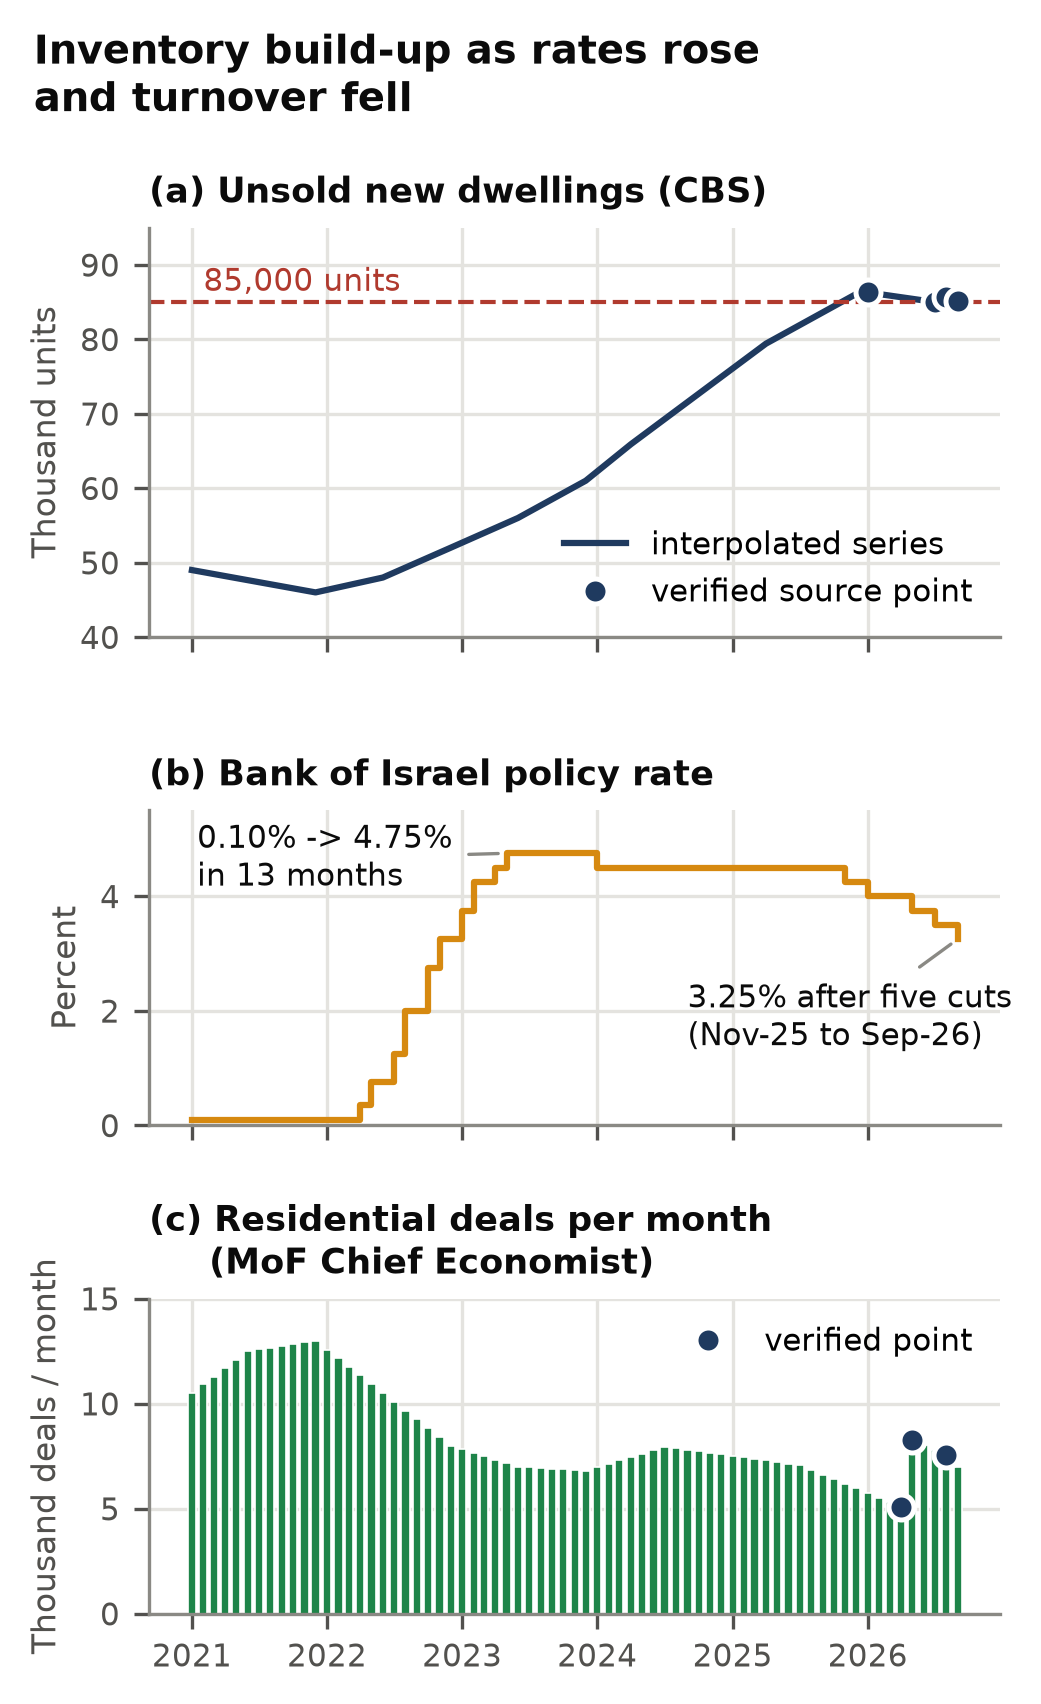
\includegraphics[width=0.6\textwidth]{figures/fig2_unsold_inventory_vs_rates.png}
\caption[מלאי לא־מכור, ריבית בנק ישראל ועסקאות, \en{2021–2026}]{מלאי הדירות החדשות שלא נמכרו, ריבית בנק ישראל ומספר העסקאות החודשי, \en{2021–2026}. הנקודות הן ערכים שאומתו מול המקור; הקו המחבר ביניהן הוא אינטרפולציה לינארית הכוללת עוגנים שטרם אומתו, ומוצג להמחשה בלבד. המלאי אינו מנוכה עונתיות, ולכן בסוף \en{2025} הוא גבוה מכ־\en{83,000} (בניכוי עונתיות) שבדוח בנק ישראל \cite{boi_annual2025_housing}}
\label{fig:inventory-rates}
\end{figure}

דירה לא־מכורה היא הון יזמי קשור הנושא עלויות מימון, ולפי \en{H3} המלאי הוא מוקד הסיכון המערכתי, כבספרד (סעיף~\ref{sec:ch2-spain}); מגבלת הספירה צוינה בסעיף~\ref{sec:ch1-scope}.

במקביל גדל מינוף היזמים. לפי בנק ישראל, עלה האשראי הבנקאי לפרויקטים של מגורים מכ־\nis{49} מיליארד בשנת \en{2024} לכ־\nis{69} מיליארד בשנת \en{2025} \cite{boi2026_recredit,boi2026_resloans}, וענפי הבינוי והנדל״ן מהווים כ־\pct{39} מהאשראי העסקי של הבנקים (\en{2025}) \cite{boi2026_recredit}.

\subsection{גודל השוק: \en{TAM}, \en{SAM} ו־\en{SOM}}
\label{sec:ch3-tam}

\subsubsection{הגדרת הרמות}
\label{sec:ch3-tam-def}
\begin{sloppypar}\noindent המודל, השאול מניתוח שווקים, מתחם את החשיפה: \mbox{\en{TAM (Total Addressable Market)}} הוא כלל השוק: הדירות והביקוש; \mbox{\en{SAM (Serviceable Available Market)}} הוא השוק הרלוונטי: בנייה חדשה; \mbox{\en{SOM (Serviceable Obtainable Market)}} הוא מוקד החשיפה: המלאי הלא־מכור והעסקאות הנדחות. טבלה~\ref{tab:ch3-tam} מפרידה בין מלאי (מצב בנקודת זמן) לזרם (לתקופה); המועדים שונים, ולכן לא חושבו יחסים בין הרמות.\end{sloppypar}

\begin{table}[!htb]
\centering
\caption{\en{TAM}, \en{SAM} ו־\en{SOM} בשוק הדיור בישראל (יחידות דיור)}
\label{tab:ch3-tam}
\footnotesize
\begin{tabularx}{\tabmaxwidth}{>{\raggedleft\arraybackslash}p{2.4cm} >{\hsize=.85\hsize}R >{\hsize=1.15\hsize}R}
\toprule
\hd{רמה ואוכלוסייה} & \hd{מלאי (תאריך)} & \hd{זרם (תקופה)} \\
\midrule
\en{TAM}: כלל הדירות והביקוש & כ־\en{3.02} מיליון דירות (אמצע \en{2025}) \cite{cbs_stock_2025} & צורך דמוגרפי של כ־\en{65,500} בשנה (\en{2026–2035}); כ־\en{90,700} עסקאות (\en{2025}) \cite{boi_annual2025_housing} \\
\midrule
\en{SAM}: בנייה חדשה & \en{217,200} בבנייה פעילה (סוף יוני \en{2026}) \cite{cbs_construction_2026q2} & כ־\en{34,000} דירות חדשות נמכרו (\en{2025}) \cite{boi_annual2025_housing}; \en{9,190} ברבעון השלישי של \en{2026} \cite{cbs_newdwellings_2026q3} \\
\midrule
\en{SOM-1}: דירות לא־מכורות & \en{85,080} (סוף ספטמבר \en{2026}) \cite{cbs_newdwellings_2026q3} & \en{25.8} חודשי היצע \cite{cbs_newdwellings_2026q3}; נגזר: \mbox{\en{85,080 / 25.8 ≈ 3,300}} מכירות בחודש \\
\midrule
\en{SOM-2}: עסקאות בתשלום נדחה & לא אותר נתון רשמי & \pct{30} ממכירות הקבלנים בחמישה אזורים (אוגוסט \en{2026}) \cite{mof_review_2026_08}; אומדן: \en{373–622} בחודש (הנחה) \\
\bottomrule
\end{tabularx}
\end{table}

\subsubsection{חפיפות, אומדן ומגבלות}
\label{sec:ch3-tam-limits}
\en{SOM-1} ו־\en{SOM-2} הן \textbf{אוכלוסיות שונות שאין לחבר}: דירה לא־מכורה חסרה רוכש (סיכון ליזם), ועסקה נדחית היא דירה שנמכרה ונגרעה מן המלאי (סיכון לרוכש); ביטול עסקה מחזיר אותה אליו. גם הרמות אינן מקוננות במלואן: מלאי הלמ״ס נספר מקבלת ההיתר \cite{boi_annual2025_housing}, ולכן חלק מ־\en{SOM-1} אינו בבנייה פעילה, ואילו \en{SAM} כולל דירות שאינן למכירה. אומדן \en{SOM-2} נשען על \en{2,072} מכירות קבלנים בשוק החופשי באוגוסט \cite{mof_review_2026_08}: בחמשת האזורים, המרכזים כ־\pct{60} מהמכירות, \mbox{\en{2,072 × 0.60 × 0.30 ≈ 373}}; בהנחה לא מאומתת ששכיחות זהה חלה בכל הארץ, \mbox{\en{2,072 × 0.30 ≈ 622}}. בשכיחות של מאי (\pct{20}) הטווח הוא \en{249–414}. זהו אומדן יתר: ה־\pct{30} חל רק על מסירה של שנה ומעלה, וההטבות אינן בהכרח \deal{20/80}. המלאי המצטבר של \en{SOM-2} אינו ידוע.

\section{מבצעי המימון הקבלניים}
\label{sec:ch3-promotions}

הורדת מחיר גלויה הייתה פוגעת בערך המלאי והבטוחות. במקומה אימץ הענף הסדרי תשלום שמעניקים לרוכש הטבה כלכלית בלי לשנות את מחיר המחירון המדווח \cite{boi_fsr2024h2,boi_circular2816}:
\begin{itemize}
  \item \textbf{מבצע \deal{20/80}:} כ־\pct{20} בחתימה ויתרת ה־\pct{80} במסירה, לרוב כעבור שלוש עד ארבע שנים (בגרסאות קיצוניות \deal{10/90}), בדרך כלל ללא הצמדה למדד תשומות הבנייה.
  \item \textbf{מבצע \deal{20/50/30}:} \pct{20} בחתימה, \pct{50} בשלב ביניים ו־\pct{30} במסירה; התפשט במיוחד לאחר התערבות בנק ישראל.
  \item \textbf{הלוואת בלון במימון היזם:} הלוואה בנקאית שהקרן שלה נפרעת בסוף התקופה, והיזם משלם את הריבית, כולה או חלקה, בתקופת הבנייה.
\end{itemize}
איור~\ref{fig:credit-triangle} מציג את הזרמים בין הצדדים.

\begin{figure}[!htb]
\centering
% =====================================================================
%  figures/tikz_credit_triangle.tex — Buyer / Developer / Lending bank:
%  money flows and risk transfers in 20/80 and 20/50/30 deals.
%  Built in an English (LTR) environment; Hebrew labels wrapped in \he{}
%  (BiDi rule 6). NOTE: no `text width` on Hebrew nodes — automatic
%  wrapping of RTL text inside TikZ nodes is mis-measured under LuaLaTeX;
%  every line break is explicit (\\). Usage in a chapter:
%    \begin{figure}[htbp]\centering
%      % =====================================================================
%  figures/tikz_credit_triangle.tex — Buyer / Developer / Lending bank:
%  money flows and risk transfers in 20/80 and 20/50/30 deals.
%  Built in an English (LTR) environment; Hebrew labels wrapped in \he{}
%  (BiDi rule 6). NOTE: no `text width` on Hebrew nodes — automatic
%  wrapping of RTL text inside TikZ nodes is mis-measured under LuaLaTeX;
%  every line break is explicit (\\). Usage in a chapter:
%    \begin{figure}[htbp]\centering
%      \input{figures/tikz_credit_triangle.tex}
%      \caption{משולש האשראי: זרמי כסף וסיכון בעסקאות \en{20/80} ו־\en{20/50/30}}
%      \label{fig:credit-triangle}
%    \end{figure}
% =====================================================================
\begin{english}
\begin{tikzpicture}[
  font=\small,
  actor/.style={rectangle, rounded corners=4pt, draw=brandNavy, line width=1pt,
    fill=brandPale, align=center, minimum width=3.9cm, minimum height=1.9cm,
    drop shadow={opacity=0.15}},
  money/.style={-{Stealth[length=3mm]}, line width=1.3pt, brandGreen!85!black},
  risk/.style={-{Stealth[length=3mm]}, line width=1.3pt, brandRed, dashed},
  guar/.style={-{Stealth[length=3mm]}, line width=1.1pt, brandSteel, densely dotted},
  lbl/.style={fill=white, inner sep=2pt, align=center, font=\footnotesize},
]
% --- actors (Hebrew reading order: buyer on the right) ---
\node[actor] (buyer) at (9.0,0)
  {\he{\textbf{הרוכש}}\\[2pt]\he{משלם \pct{20} הון עצמי}\\\he{היתרה נדחית למסירה}};
\node[actor] (dev) at (0,0)
  {\he{\textbf{היזם / הקבלן}}\\[2pt]\he{סופג ריבית והצמדה}\\\he{ממונף בליווי בנקאי}};
\node[actor, fill=gray!8] (bank) at (4.5,6.3)
  {\he{\textbf{הבנק המלווה}}\\[2pt]\he{ליווי סגור ומשכנתא}\\\he{(לעיתים הלוואת בלון)}};

% --- deal-structure badge ---
\node[draw=brandNavy, fill=white, rounded corners=3pt, align=center, font=\footnotesize,
      inner sep=4pt] at (4.5,3.1)
  {\he{\textbf{מבנה העסקה}}\\[3pt]
   \en{\textbf{20/80}}\\
   \he{\pct{20} בחתימה, \pct{80} במסירה}\\[3pt]
   \en{\textbf{20/50/30}}\\
   \he{\pct{20} בחתימה, \pct{50} בבנייה,}\\
   \he{\pct{30} במסירה}};

% --- Buyer <-> Developer (bottom edge) ---
\draw[money] ([yshift=4mm]buyer.west) -- node[lbl, above=1mm]{\he{מקדמה של \pct{20} בחתימה}} ([yshift=4mm]dev.east);
\draw[risk]  ([yshift=-4mm]dev.east) -- node[lbl, below=1mm]
  {\he{סבסוד ריבית והצמדה (הנחה סמויה)}\\\he{סיכון ביטול עסקה}} ([yshift=-4mm]buyer.west);

% --- Bank <-> Developer (left edge) ---
\draw[money] ([xshift=6mm]bank.south west) -- coordinate[pos=0.22] (lm) ([xshift=8mm]dev.north);
\draw[risk]  ([xshift=-2mm]dev.north) -- coordinate[pos=0.3] (lr) ([xshift=-4mm]bank.south west);

% --- Bank <-> Buyer (right edge) ---
\draw[money] ([xshift=-6mm]bank.south east) -- coordinate[pos=0.22] (rm) ([xshift=-8mm]buyer.north);
\draw[guar]  ([xshift=2mm]buyer.north) -- coordinate[pos=0.3] (rg) ([xshift=4mm]bank.south east);

% --- side labels drawn last so their white fill sits above all arrows ---
\node[lbl, left=2mm, text=brandGreen!70!black] at (lm) {\he{ליווי פיננסי}\\\he{(אשראי לבנייה)}};
\node[lbl, left=2mm, text=brandRed] at (lr) {\he{ריכוזיות אשראי;}\\\he{כשל יזם פוגע בתיק}};
\node[lbl, right=2mm, text=brandGreen!70!black] at (rm) {\he{משכנתא / הלוואת בלון}\\\he{על \pct{80} או \pct{30} במסירה}};
\node[lbl, right=2mm, text=brandSteel] at (rg) {\he{ערבות חוק המכר;}\\\he{סיכון סירוב מימון במסירה}};

% --- legend ---
\begin{scope}[shift={(0,-2.4)}, font=\footnotesize]
  \draw[money] (8.6,0) -- (9.6,0); \node[anchor=east] at (8.5,0) {\he{זרם כספי}};
  \draw[risk]  (5.4,0) -- (6.4,0); \node[anchor=east] at (5.3,0) {\he{העברת סיכון}};
  \draw[guar]  (1.9,0) -- (2.9,0); \node[anchor=east] at (1.8,0) {\he{ערבות / תלות}};
\end{scope}
\end{tikzpicture}
\end{english}

%      \caption{משולש האשראי: זרמי כסף וסיכון בעסקאות \en{20/80} ו־\en{20/50/30}}
%      \label{fig:credit-triangle}
%    \end{figure}
% =====================================================================
\begin{english}
\begin{tikzpicture}[
  font=\small,
  actor/.style={rectangle, rounded corners=4pt, draw=brandNavy, line width=1pt,
    fill=brandPale, align=center, minimum width=3.9cm, minimum height=1.9cm,
    drop shadow={opacity=0.15}},
  money/.style={-{Stealth[length=3mm]}, line width=1.3pt, brandGreen!85!black},
  risk/.style={-{Stealth[length=3mm]}, line width=1.3pt, brandRed, dashed},
  guar/.style={-{Stealth[length=3mm]}, line width=1.1pt, brandSteel, densely dotted},
  lbl/.style={fill=white, inner sep=2pt, align=center, font=\footnotesize},
]
% --- actors (Hebrew reading order: buyer on the right) ---
\node[actor] (buyer) at (9.0,0)
  {\he{\textbf{הרוכש}}\\[2pt]\he{משלם \pct{20} הון עצמי}\\\he{היתרה נדחית למסירה}};
\node[actor] (dev) at (0,0)
  {\he{\textbf{היזם / הקבלן}}\\[2pt]\he{סופג ריבית והצמדה}\\\he{ממונף בליווי בנקאי}};
\node[actor, fill=gray!8] (bank) at (4.5,6.3)
  {\he{\textbf{הבנק המלווה}}\\[2pt]\he{ליווי סגור ומשכנתא}\\\he{(לעיתים הלוואת בלון)}};

% --- deal-structure badge ---
\node[draw=brandNavy, fill=white, rounded corners=3pt, align=center, font=\footnotesize,
      inner sep=4pt] at (4.5,3.1)
  {\he{\textbf{מבנה העסקה}}\\[3pt]
   \en{\textbf{20/80}}\\
   \he{\pct{20} בחתימה, \pct{80} במסירה}\\[3pt]
   \en{\textbf{20/50/30}}\\
   \he{\pct{20} בחתימה, \pct{50} בבנייה,}\\
   \he{\pct{30} במסירה}};

% --- Buyer <-> Developer (bottom edge) ---
\draw[money] ([yshift=4mm]buyer.west) -- node[lbl, above=1mm]{\he{מקדמה של \pct{20} בחתימה}} ([yshift=4mm]dev.east);
\draw[risk]  ([yshift=-4mm]dev.east) -- node[lbl, below=1mm]
  {\he{סבסוד ריבית והצמדה (הנחה סמויה)}\\\he{סיכון ביטול עסקה}} ([yshift=-4mm]buyer.west);

% --- Bank <-> Developer (left edge) ---
\draw[money] ([xshift=6mm]bank.south west) -- coordinate[pos=0.22] (lm) ([xshift=8mm]dev.north);
\draw[risk]  ([xshift=-2mm]dev.north) -- coordinate[pos=0.3] (lr) ([xshift=-4mm]bank.south west);

% --- Bank <-> Buyer (right edge) ---
\draw[money] ([xshift=-6mm]bank.south east) -- coordinate[pos=0.22] (rm) ([xshift=-8mm]buyer.north);
\draw[guar]  ([xshift=2mm]buyer.north) -- coordinate[pos=0.3] (rg) ([xshift=4mm]bank.south east);

% --- side labels drawn last so their white fill sits above all arrows ---
\node[lbl, left=2mm, text=brandGreen!70!black] at (lm) {\he{ליווי פיננסי}\\\he{(אשראי לבנייה)}};
\node[lbl, left=2mm, text=brandRed] at (lr) {\he{ריכוזיות אשראי;}\\\he{כשל יזם פוגע בתיק}};
\node[lbl, right=2mm, text=brandGreen!70!black] at (rm) {\he{משכנתא / הלוואת בלון}\\\he{על \pct{80} או \pct{30} במסירה}};
\node[lbl, right=2mm, text=brandSteel] at (rg) {\he{ערבות חוק המכר;}\\\he{סיכון סירוב מימון במסירה}};

% --- legend ---
\begin{scope}[shift={(0,-2.4)}, font=\footnotesize]
  \draw[money] (8.6,0) -- (9.6,0); \node[anchor=east] at (8.5,0) {\he{זרם כספי}};
  \draw[risk]  (5.4,0) -- (6.4,0); \node[anchor=east] at (5.3,0) {\he{העברת סיכון}};
  \draw[guar]  (1.9,0) -- (2.9,0); \node[anchor=east] at (1.8,0) {\he{ערבות / תלות}};
\end{scope}
\end{tikzpicture}
\end{english}

\caption{משולש האשראי: זרמי כסף וסיכון בעסקאות \en{20/80} ו־\en{20/50/30}}
\label{fig:credit-triangle}
\end{figure}

\paragraph{מחיר מחירון מול מחיר כלכלי.} דחיית תשלום של \pct{80} מהמחיר, ללא הצמדה וללא ריבית, שקולה להנחה במונחי ערך נוכחי. בתרחיש להמחשה, עם דחייה של שלוש שנים, ההנחה הגלומה היא \en{10.9\%–12.8\%} בשיעורי היוון של \en{5\%–6\%} (פרק~\ref{ch:methodology}), והיא גדלה עוד כשהיזם מממן גם את ריבית הבלון. ההנחה אינה מתבטאת במדד המחירים הרשמי (הנחת יסוד \en{2}, סעיף~\ref{sec:ch1-scope}), וזהו המנגנון שהשערה \en{H1} מכנה \textbf{קשיחות מחירים מלאכותית}. שכיחות ההטבות עלתה מ־\pct{20} במאי ל־\pct{30} באוגוסט \en{2026} (סעיף~\ref{sec:ch3-tam}) \cite{mof_review_2026_08,nadlancenter_2026_08_promos}. ריכוז העסקאות בשנים \en{2023–2025} ומשך בנייה של שלוש עד ארבע שנים מרכזים את המסירות בשנים \en{2026–2027}: ״קיר המסירות״.

\section{התערבות בנק ישראל}
\label{sec:ch3-boi}

בדוחות היציבות הפיננסית לשנת \en{2024} הצביע בנק ישראל על סיכוני המבצעים: דחיית מבחני הזכאות, טשטוש המחירים ותלות היזמים במכירות ובאשראי \cite{boi_fsr2024h1,boi_fsr2024h2}. ב־\en{23} במרץ \en{2025} פרסם בנק ישראל טיוטת הוראת שעה \cite{mof_review_2026_08}, וב־\en{6} באפריל \en{2025} פורסם חוזר מס׳ \en{2816}, שנכנס לתוקף ביום פרסומו \cite{boi_circular2816}:
\begin{enumerate}
  \item \textbf{תיקון הוראה \en{203} (משקל סיכון):} אשראי לליווי פרויקט מגורים שבו שיעור החוזים הדוחים ״חלק מהותי״ מהמחיר עולה על \pct{25} ישוקלל במשקל סיכון של \pct{150}. ״חלק מהותי״ מוגדר כסכום שהרוכש רשאי לדחות למסירה ועולה על \pct{40} ממחיר הדירה.
  \item \textbf{סעיף \en{8}א בהוראה \en{329}:} היקף הלוואות הבולט והבלון שהריבית עליהן מסובסדת בידי היזם לא יעלה על \pct{10} מסך ביצועי הלוואות הדיור של הבנק ברבעון קלנדרי.
\end{enumerate}
החוזר הוגדר כהוראת שעה שתוקפה עד \en{31} בדצמבר \en{2026}, והארכתה תיבחן ״בבוא העת״ \cite{boi_circular2816}; עד נובמבר \en{2026} לא אותרה החלטה רשמית בעניין.

\paragraph{תגובת השוק.} המבצעים לא נעלמו, אלא שינו צורה: יזמים רבים עברו ממבני \deal{20/80} למבנים מדורגים כגון \deal{20/50/30}, ואחרים הציעו מימון ריבית ישיר ואשראי חוץ־בנקאי, כצפוי מתאוריית בנקאות הצל (סעיף~\ref{sec:ch1-theory}) \cite{pozsar2010}.

\paragraph{לקראת ״קיר המסירות״.}\label{sec:ch3-wall} \textbf{הרוכשים} יידרשו לשלם \en{30\%–80\%} מהמחיר במשכנתא שתיבחן במלוא מבחני \en{LTV} ו־\en{PTI}, בריבית גבוהה בהרבה מזו של \en{2021} ובשמאות שאולי תפחת ממחיר החוזה (\en{H2}). \textbf{היזמים} תלויים בגביית היתרות, במכירת המלאי ובמחזור החוב (\en{H3}). \textbf{הבנקים} חשופים לשני הצדדים, אך מוגנים בחוק המכר, בליווי הסגור ובחבות אישית מלאה \cite{salelaw1974,boi_directive329}.

\section{מאמר הדגל ופער הידע}
\label{sec:ch3-flagship}

\paragraph{מאמר הדגל.} מאמר הדגל של העבודה הוא \en{Mian \& Sufi (2009), ``The Consequences of Mortgage Credit Expansion''} \cite{mian2009}, והוא עומד בשלושה קריטריונים: (\en{1}) \textbf{פרסום בכתב עת שפיט מוביל}, \en{The Quarterly Journal of Economics}; (\en{2}) \textbf{רלוונטיות ישירה}: הוא מבחין בין עליית מחירים הנובעת מיסודות כלכליים לבין עלייה הנובעת מהתרחבות היצע האשראי, וזו ההבחנה ש־\en{H1} בוחנת בישראל; (\en{3}) \textbf{אפשרות שחזור}: הוא נשען על נתונים מנהליים ברמת המיקוד ועל אסטרטגיית זיהוי מתועדת הניתנת לשחזור על נתוני רשות המסים והלמ״ס. מגבלתו בהקשר הישראלי היא שאין בו ערוץ שבו היזם עצמו מעניק את האשראי ודוחה את מבחן היכולת; מכאן מודל \en{NPV} ומבחני הקיצון (פרק~\ref{ch:methodology}).

\begin{keyfinding}[פער הידע]
לא אותר במחקר הקיים אומדן כמותי לפער שבין מחיר המחירון לבין הערך הנוכחי של עסקאות המימון הקבלניות בישראל, ולהשפעתו על יכולת ההחזר של הרוכשים ועל חוסן היזמים והבנקים ב״קיר המסירות״ של \en{2026–2027}.
\end{keyfinding}

פער זה והדמיון החלקי לארה״ב ולספרד מחייבים את ההשוואה שבפרק הבא.

% =====================================================================
% פרק 4 — ניתוח השוואתי: ארה״ב 2007/08, ספרד 2007/08 וישראל 2022–2026
% RESEARCH_CORE_AGENT (Agent 2)
% =====================================================================
\chapter{ניתוח השוואתי: ארה״ב, ספרד וישראל}
\label{ch:comparative}

\begin{managerbox}
השאלה אם ישראל ״חוזרת על \en{2008}״ היא שאלה של מנגנונים ולא של דמיון כללי. מנהל בבנק, ביזמות או ברגולציה צריך לדעת אילו מנגנוני כשל של ארה״ב ושל ספרד קיימים בישראל, באיזו עוצמה, ואילו בלמים מוסדיים חסרו שם וקיימים כאן. פרק זה משווה את שלושת המקרים לפי אותם פרמטרים, ומכוון את מבחני הקיצון שבפרק~\ref{ch:delivery-wall} לנקודות התורפה.
\end{managerbox}

\section{מסגרת ההשוואה וטבלת הפרמטרים}
\label{sec:ch4-table}

ההשוואה מפורקת לממדים התואמים את מנגנוני הכשל שבטבלה~\ref{tab:ch2-mechanisms}: מבנה המוצר וזעזוע התשלום, מינוף משקי הבית, מינוף היזמים, מבנה המימון של הבנקים ורשתות הביטחון המוסדיות. נתונים רשמיים מוצגים עם מקור; ערכים מכוילים (מסוגננים, לסדר גודל) מסומנים בכוכבית ומשמשים להמחשה בלבד. טבלה~\ref{tab:ch4-comparison} מרכזת את שלושת המקרים לפי עשרה פרמטרים: ישראל דומה לארה״ב רק בדחיית מבחן היכולת של הרוכש, ולספרד בממד היזמי והבנקאי, ושונה משתיהן במינוף משקי הבית, באיגוח וברגולציה.

\begin{table}[!htb]
\centering
\caption[השוואה רב־פרמטרית: ארה״ב, ספרד וישראל]{השוואה רב־פרמטרית: ארה״ב \en{2007/08}, ספרד \en{2007/08} וישראל \en{2022–2026}}
\label{tab:ch4-comparison}
\small
\begin{tabularx}{\tabmaxwidth}{>{\raggedleft\arraybackslash}p{2.6cm} R R R}
\toprule
\hd{פרמטר} & \hd{ארה״ב \en{2007/08}} & \hd{ספרד \en{2007/08}} & \hd{ישראל \en{2022–2026}} \\
\midrule
מוצר דחיית התשלום & \en{Teaser/ARM}, \en{Interest-Only} \cite{fcic2011} & משכנתאות בריבית משתנה; אין מוצר דחייה ייחודי \cite{akin2014} & \deal{20/80}, \deal{20/50/30}, בלון במימון היזם \cite{boi_circular2816} \\
\midrule
מפעיל הזעזוע & איפוס ריבית ועצירת המימון מחדש \cite{mayer2009} & אבטלה וירידת מחירים \cite{akin2014} & משכנתא בריבית ובשמאות של יום המסירה \cite{boi2026_resloans} \\
\midrule
מגבלות \en{LTV/PTI} & חלשות; תיעוד חסר נפוץ \cite{mayer2009} & -- & \en{LTV} עד \pct{75}; \en{PTI} עד \pct{50} \cite{boi_directive329} \\
\midrule
חוב משקי הבית לתוצר & \pct{98.4} (\en{2007Q4}) \cite{bis_hhdebt} & כ־\pct{82}* & \pct{42.5} (\en{2025}) \cite{bis_hhdebt} \\
\midrule
\en{LTV} אפקטיבי & \pct{95}* & \pct{85}* & \pct{85}* \\
\midrule
חשיפת האשראי הבנקאי לנדל״ן & \pct{55}* & \pct{60}* & \pct{39} מהאשראי העסקי \cite{boi2026_recredit} \\
\midrule
מינוף המתווכים & בנקי השקעות עד \en{40:1} \cite{fcic2011} & קופות חיסכון אזוריות \cite{akin2014} & מאזן בנקאי מפוקח \cite{boi2026_recredit} \\
\midrule
מבנה המימון & הפקה לשם הפצה, \en{MBS/CDO} \cite{keys2010} & בעיקר במאזן \cite{akin2014} & במאזן; חוק איגוח טרם הושלם \cite{boi_survey2025,hapoalim_q3_2026} \\
\midrule
חבות הלווה & \en{Non-Recourse} בחלק מהמדינות \cite{ghent2011} & -- & חבות אישית מלאה (פרק~\ref{ch:israel}) \\
\midrule
עלות המשבר למערכת & כ־\en{4} מיליון משפחות איבדו את ביתן \cite{fcic2011} & \en{€60.6} מיליארד (\pct{5.6} תוצר) \cite{bde2017note} & טרם התממש \\
\bottomrule
\end{tabularx}

\vspace{2pt}
{\footnotesize * ערך מכויל ומסוגנן (להמחשה), אינו נתון נצפה; ״--״: לא נמצא נתון מאומת.}
\end{table}

\section{ניתוח המנגנונים}
\label{sec:ch4-mechanisms}

\paragraph{זעזוע התשלום: \en{Teaser/ARM} מול \deal{20/80}.}\label{subsec:ch4-shock}
המכנה המשותף של מוצרי ה־\en{Teaser/ARM} ושל מבצעי המימון הוא דחיית מבחן היכולת. בארה״ב כרבע מהמשכנתאות במחצית הראשונה של \en{2005} היו ״ריבית בלבד״ \cite{fcic2011}. בישראל הפער הממוצע בין חתימת העסקה לנטילת המשכנתא התרחב מכחצי שנה בשנים \en{2018–2022} לכשמונה חודשים ב־\en{2025}, בין היתר בעקבות תמריצי המימון של היזמים \cite{boi2026_resloans}.

עם זאת, קיימים שני הבדלים מהותיים. ראשית, בארה״ב הלווה כבר החזיק במשכנתא והזעזוע נבע מאיפוס הריבית, ואילו בישראל הרוכש ייבחן במבחני הוראה \en{329} (סעיף~\ref{sec:ch3-baseline}) ביום המסירה: המבחן נדחה אך לא בוטל. שנית, מאייר, פנס ושרלונד מראים כי עד אמצע \en{2008} המוצרים הלא־קונבנציונליים לא היו גורם מרכזי לחדלות הפירעון; הגורמים העיקריים היו ירידת המחירים והידרדרות החיתום \cite{mayer2009}. מכאן שהסיכון בישראל אינו במבנה המבצע עצמו, אלא באפשרות שביום המסירה המימון לא יהיה זמין בתנאים הדרושים. בתרחיש להמחשה, ההחזר החודשי עולה בכ־\pct{29} באיפוס \en{Teaser} ובכ־\pct{76} במעבר מתשלום ריבית בלבד במבנה \deal{20/50/30} למשכנתא מלאה (איור~\ref{fig:payment-shock}).

\paragraph{מינוף משקי הבית ומינוף נסתר.}\label{sec:ch4-hidden}
חוב משקי הבית ביחס לתוצר בישראל נמוך ממחצית רמתו בארה״ב ב־\en{2007} (טבלה~\ref{tab:ch4-comparison}). בארה״ב חוב זה היה ערוץ ההעברה המרכזי ממשבר הדיור לכלכלה הריאלית \cite{mian2009,mian2014}, ובישראל ערוץ זה חלש בהרבה. אולם המינוף המצרפי עשוי להסתיר מינוף גבוה ברמת העסקה. איור~\ref{fig:ch4-comparative-risk} מראה שה־\en{LTV} המדווח בישראל נמוך משל ארה״ב וספרד, אך ה־\en{LTV} האפקטיבי, המחושב על המחיר הכלכלי ולא על מחיר המחירון, מתקרב לרמה הספרדית. בתרחיש המחקר, משכנתא של \pct{75} על דירה שמחירה הכלכלי נמוך בכ־\pct{12} ממחיר המחירון (משוואה~\ref{eq:ch5-npv}) שקולה ל־\en{LTV} אפקטיבי של כ־\pct{85} (\en{0.75/0.88}). כל הערכים באיור מכוילים, למעט יחס החוב לתוצר בארה״ב ובישראל וחשיפת הבנקים בישראל.

\begin{figure}[!htb]
\centering
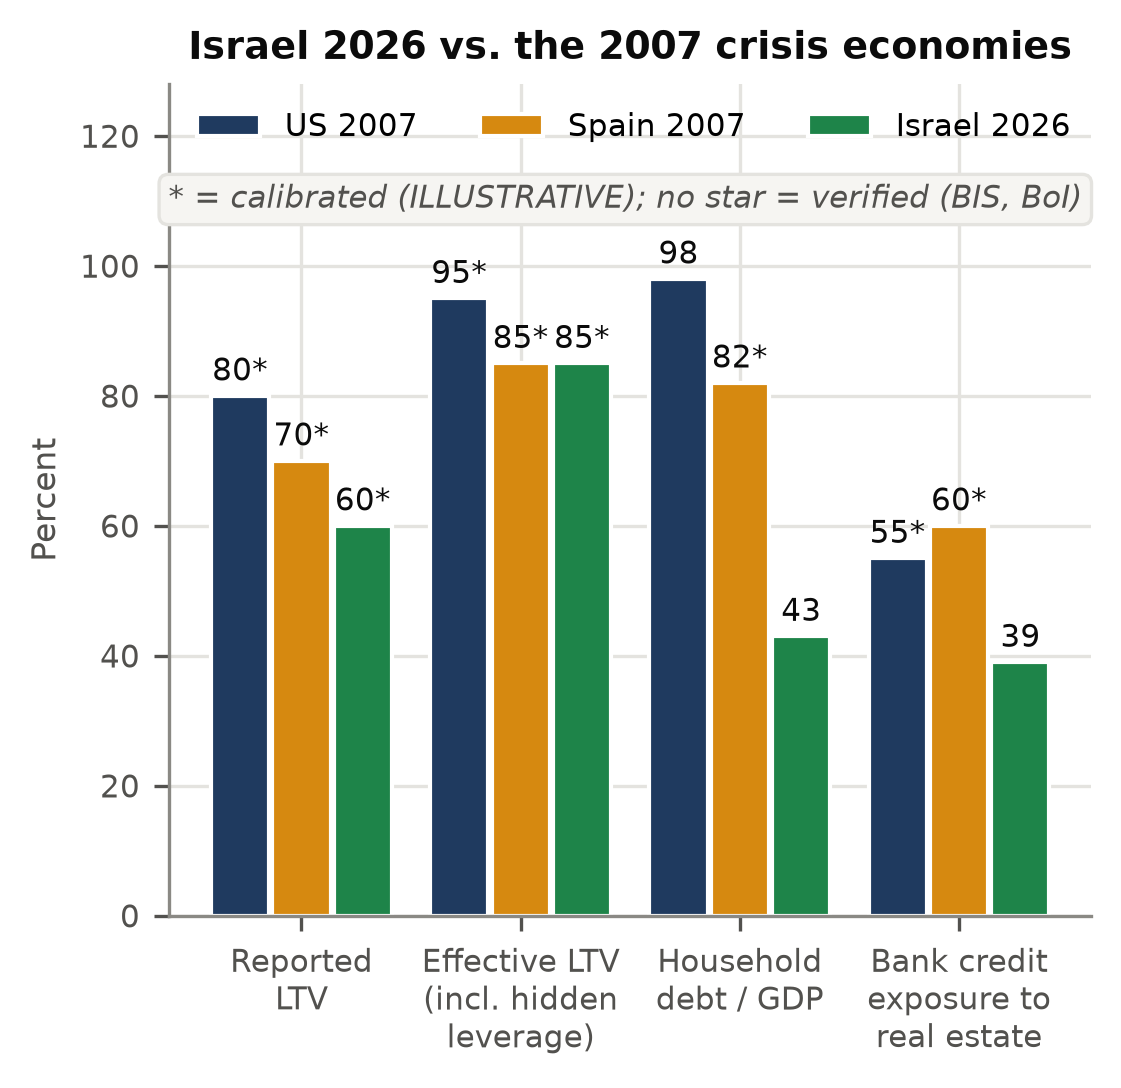
\includegraphics[width=0.65\textwidth]{figures/fig6_comparative_risk_2008_vs_2026.png}
\caption[השוואת מדדי סיכון: ארה״ב וספרד \en{2007} מול ישראל \en{2026}]{השוואת מדדי סיכון: ארה״ב \en{2007}, ספרד \en{2007} וישראל \en{2026}. ערכים המסומנים בכוכבית מכוילים להמחשה; החוב לתוצר בארה״ב ובישראל לפי \en{BIS}, וחשיפת הבנקים בישראל לפי בנק ישראל}
\label{fig:ch4-comparative-risk}
\end{figure}

\paragraph{מינוף היזמים וחשיפת הבנקים: הקבלה לספרד.}\label{subsec:ch4-developers}
בממד היזמי ספרד היא נקודת ההשוואה הקרובה ביותר: האשראי לבינוי ולנדל״ן הוזרם בעיקר דרך קופות החיסכון, ומשבר הנדל״ן הפך למשבר בנקאי גם ללא מוצרי משכנתא אקזוטיים \cite{akin2014}, בעלות משאבים נטו (ציבוריים ופרטיים) של כ־\en{€60.6} מיליארד (\pct{5.6} מהתוצר) עד סוף \en{2015} \cite{bde2017note}. בישראל, האשראי לענף הבינוי והנדל״ן מהווה כ־\pct{39} מהאשראי העסקי המאזני וכ־\pct{21} מהאשראי לציבור, והוא צמח ב־\en{2025} בכ־\pct{14} (האשראי לפרויקטים למגורים: כ־\pct{40}) \cite{boi2026_recredit}. זהו המנגנון שאפיין את ספרד: בנייה שמקדימה את המכירות ובנקים שחשיפתם לענף גדלה. ההבדל הוא במבנה: האשראי לפרויקטים ניתן בליווי סגור. אולם גם בישראל האשראי לקרקע למגורים (\nis{81} מיליארד, סוף \en{2025}) גדול מהאשראי לפרויקטים (\nis{69} מיליארד) \cite{boi_survey2025}.

\paragraph{מבנה המימון ורשתות הביטחון.}\label{subsec:ch4-safety}
בארה״ב ניתק מודל ״ההפקה לשם הפצה״ את המלווה מהסיכון \cite{keys2010}, ובנקי ההשקעות פעלו במינוף של עד \en{40:1} \cite{fcic2011}. בישראל האשראי מוחזק במאזני הבנקים: התמריץ לחתום בקפדנות נשמר, אך הסיכון מרוכז במערכת הבנקאית, כמו בספרד. שלושה בלמים מוסדיים מבדילים את ישראל. \textbf{חבות הלווה}: גנט וקודליאק מצאו שבמדינות ללא חבות אישית לווים נטו יותר לחדלות פירעון \cite{ghent2011}; בישראל החבות מלאה, ולכן ״פירעון אסטרטגי״ אינו צפוי. \textbf{ערבויות חוק המכר} מגנות על הרוכש מפני קריסת היזם \cite{salelaw1974}, אך מעבירות את הסיכון לבנק הערב, וערוץ זה נכלל במבחן הקיצון (משוואה~\ref{eq:ch5-coverage}). \textbf{מדיניות מאקרו־יציבותית}: ההפרשות הדינמיות בספרד מיתנו את מחזור האשראי \cite{jimenez2017} אך לא מנעו את המשבר \cite{bde2017}; בישראל פועלות הוראה \en{329} וחוזר \en{2816} (סעיפים~\ref{sec:ch3-baseline} ו־\ref{sec:ch3-boi}). הלקח הספרדי הוא שכלים אלה מצמצמים את הנזק, אך אינם מחליפים הגבלה של ריכוז החשיפה לענף אחד.

\section{מפת השחזור}
\label{sec:ch4-replication}

איור~\ref{fig:ch4-radar} מסכם את ההשוואה במפת עוצמה של שישה מנגנוני כשל, בסולם \en{1} (חלש) עד \en{5} (חזק). הציונים הם הערכה איכותית של צוות המחקר על בסיס טבלה~\ref{tab:ch4-comparison}, ולא מדידה. הפרופיל הישראלי חופף לספרדי בצד היזמי והבנקאי, לאמריקאי רק בדחיית מבחן היכולת, ונמוך משניהם בסיכון מחוץ למאזן ובחולשת הרגולציה.

\begin{figure}[!htb]
\centering
\begin{english}
\begin{tikzpicture}[scale=0.8, font=\footnotesize]
  \foreach \r in {1,...,5}{
    \draw[gray!35] (90:\r*0.5) -- (30:\r*0.5) -- (-30:\r*0.5) -- (-90:\r*0.5) -- (-150:\r*0.5) -- (150:\r*0.5) -- cycle;
  }
  \foreach \a in {90,30,-30,-90,-150,150}{ \draw[gray!50] (0,0) -- (\a:2.5); }
  \foreach \r in {1,...,5}{ \node[gray, font=\scriptsize, anchor=west] at (0.05,\r*0.5) {\r}; }
  \node[anchor=south] at (90:2.6) {\he{דחיית מבחן היכולת}};
  \node[anchor=west]  at (30:2.6) {\he{מינוף משקי הבית}};
  \node[anchor=west]  at (-30:2.6) {\he{מינוף יזמים ומלאי}};
  \node[anchor=north] at (-90:2.6) {\he{ריכוז חשיפת הבנקים}};
  \node[anchor=east]  at (-150:2.6) {\he{סיכון מחוץ למאזן}};
  \node[anchor=east]  at (150:2.6) {\he{חולשת רגולציה}};
  \draw[brandNavy, line width=1.2pt, fill=brandNavy, fill opacity=0.08]
    (90:5*0.5) -- (30:5*0.5) -- (-30:3*0.5) -- (-90:3*0.5) -- (-150:5*0.5) -- (150:5*0.5) -- cycle;
  \draw[brandAmber, line width=1.2pt, dashed, fill=brandAmber, fill opacity=0.08]
    (90:2*0.5) -- (30:4*0.5) -- (-30:5*0.5) -- (-90:5*0.5) -- (-150:3*0.5) -- (150:3*0.5) -- cycle;
  \draw[brandGreen, line width=1.4pt, fill=brandGreen, fill opacity=0.12]
    (90:4*0.5) -- (30:2*0.5) -- (-30:4*0.5) -- (-90:4*0.5) -- (-150:1*0.5) -- (150:1*0.5) -- cycle;
  \begin{scope}[shift={(-5.2,-3.55)}]
    \draw[brandNavy, line width=1.2pt] (0,0) -- (0.6,0); \node[anchor=west] at (0.75,0) {US 2007/08};
    \draw[brandAmber, line width=1.2pt, dashed] (3.8,0) -- (4.4,0); \node[anchor=west] at (4.55,0) {Spain 2007/08};
    \draw[brandGreen, line width=1.4pt] (7.9,0) -- (8.5,0); \node[anchor=west] at (8.65,0) {Israel 2022--26};
  \end{scope}
\end{tikzpicture}
\end{english}
\caption[מפת עוצמה של שישה מנגנוני כשל (הערכה איכותית)]{מפת עוצמה של שישה מנגנוני כשל (סולם \en{1–5}): הערכה איכותית של צוות המחקר, להמחשה, על בסיס טבלה~\ref{tab:ch4-comparison}}
\label{fig:ch4-radar}
\end{figure}

\begin{keyfinding}
מתוך שמונה מנגנוני כשל שנגזרו מטבלה~\ref{tab:ch4-comparison}, שלושה \textbf{משוחזרים} בישראל: דחיית מבחן היכולת של הרוכש \enb{H1, H2}, זעזוע תשלום במועד מרוכז ב־\en{2026–2027} (\en{H2}) ובנייה לפני מכירה במימון בנקאי (\en{H3}). שניים \textbf{משוחזרים בחלקם}: ריכוז חשיפת הבנקים לנדל״ן, הממותן בליווי סגור (\en{H3}), והסתרת המחיר הכלכלי, שהשפעתה ברמת השוק קטנה (\en{H1}). שלושה \textbf{אינם משוחזרים}: מינוף מצרפי גבוה של משקי הבית, איגוח נרחב, ופירעון אסטרטגי \enb{Strategic Default} בהלוואות ללא חבות אישית. אלה בדיוק המנגנונים שהפכו בארה״ב משבר דיור למשבר פיננסי. לכן ישראל דומה לספרד יותר מאשר לארה״ב, והשאלה המכרעת היא אם הסיכון ייעצר במאזני היזמים או יעבור לבנקים דרך ערבויות חוק המכר ואשראי הליווי; פרק~\ref{ch:delivery-wall} מראה שבתרחיש החמור הוא אינו נעצר ביזמים.
\end{keyfinding}

הפרק הבא מפרט את הנתונים והמודלים שבאמצעותם נבחנת שאלה זו.

% =====================================================================
%  ch05_methodology_and_data.tex — Agent 3 (Python_Viz)
%  Numbers: comms/data_summary.json (single source of truth).
%  Scripts: build/scripts/ (run_all.py) · Figures: build/figures/
% =====================================================================
\chapter{מתודולוגיה ונתונים}
\label{ch:methodology}

\begin{managerbox}
מנהל סיכוני אשראי בבנק או סמנכ״ל כספים בחברה יזמית נדרש להעריך את חשיפתו לגל חדלות פירעון לפני התממשותו. פרק זה מתאר אילו נתונים אומתו, אילו הנחות נוספו ומדוע נבחרה סימולציה מכוילת. ההפרדה בין עובדה לתרחיש מאפשרת להחליף הנחה אחת ולראות כיצד משתנה המסקנה.
\end{managerbox}

\section{מקורות הנתונים ועיבודם}
\label{sec:ch5-sources}

המחקר נשען על נתוני בנק ישראל, הלמ״ס, משרד האוצר וה־\en{BIS}; נתון הזמין רק בדיווח משני מסומן ככזה (טבלה~\ref{tab:ch5-sources}).

\begin{table}[!htb]
\centering
\caption{מקורות הנתונים, תקופת הכיסוי ומעמד האימות}
\label{tab:ch5-sources}
\footnotesize
\begin{tabularx}{\tabmaxwidth}{>{\raggedleft\arraybackslash}p{3.2cm} R >{\centering\arraybackslash}p{2.0cm} >{\centering\arraybackslash}p{1.9cm}}
\toprule
\hd{סדרה} & \hd{מקור} & \hd{תקופה} & \hd{מעמד} \\
\midrule
ריבית בנק ישראל & החלטות הוועדה המוניטרית \cite{boi_rate_2026_09}; ריכוז משני \cite{boi_rate_decisions} & \en{2021–2026} & רשמי (\en{2026}) ומשני \\
מלאי דירות חדשות שלא נמכרו & נתוני הלמ״ס, דרך דיווח משני \cite{cbs_newdwellings,cbs_newdwellings_2026q3} & \en{2021–2026} & משני \\
עסקאות דירות & הכלכלן הראשי, דרך דיווח משני \cite{semerenko_market,toi_housing_2026_10} & \en{2021–2026} & משני \\
מדד מחירי הדירות & הלמ״ס \cite{cbs_priceindex_2026_222,toi_housing_2026_10} & \en{2021–2026} & שינויים שנתיים אומתו \\
חוב משקי בית לתוצר & \en{BIS} \cite{bis_hhdebt} & \en{2007}, \en{2025} & רשמי, מאומת \\
אשראי ליזמים וחשיפת בנקים & סקירת מערכת הבנקאות, בנק ישראל \cite{boi2026_recredit,boi2026_resloans} & \en{2024–2025} & רשמי, מאומת \\
הון, \en{RWA} ואשראי לבינוי ונדל״ן & דוחות רבעוניים של חמש הקבוצות (טבלה~\ref{tab:ch5-banks}) & \en{30.9.2026} & רשמי, מאומת \\
שיעור מבצעי המימון & הכלכלן הראשי \cite{mof_review_2026_08,nadlancenter_2026_08_promos} & \en{2026} & רשמי; לכיול \\
\bottomrule
\end{tabularx}
\end{table}

אומתו מול המקור (נכון ל־\en{16.11.2026}; נתוני הבנקים: \en{24.11.2026}) בעיקר נקודות של \en{2026}; ערכי \en{2021–2025} במלאי ובעסקאות ורמות מדד המחירים הם עוגנים משוחזרים, ומוצגים באיורים כקו ללא סמן.

\label{sec:ch5-cleaning}כל ערך הוזן לרישום נתונים יחיד עם תג מעמד: \en{official} (מאומת), \en{official\_\allowbreak approx} (רק חלק מהנקודות אומתו) או \en{calibrated} (פרמטר שקבע החוקר). עוגנים רבעוניים הומרו לסדרה חודשית באינטרפולציה לינארית, והריבית לסדרה מדרגתית לפי מועד כניסת כל החלטה לתוקף. מדד המחירים הוצג בבסיס ינואר \en{2021 = 100} (סעיף~\ref{sec:ch3-demand}). לעסקאות משמשת הגדרת הכלכלן הראשי \cite{toi_housing_2026_10}. ערך מאומת מוצג כעובדה עם מראה מקום; כל ערך אחר, ובכלל זה תוצאות הסימולציה, מוצג כ״תרחיש״, ״להמחשה״ או ״בהנחה כי״.

\section{חלופות מתודולוגיות ומטריצת החלטה}
\label{sec:ch5-alternatives}

שאלת המחקר משלבת השוואה לאחור של מנגנוני כשל והערכה צופה פני עתיד של עמידות המערכת ב״קיר המסירות״. נבחנו שלוש חלופות: \textbf{א — אקונומטריקה של סדרות עתיות}, מודל \term{וקטור אוטו־רגרסיבי}{VAR} או פאנל המקשרים ריבית, מחירים ומלאי לשיעורי כשל היסטוריים; \textbf{ב — סימולציה מבנית מכוילת}, מודלים מפורשים (\en{NPV}, זעזוע תשלום, \term{מונטה קרלו}{Monte Carlo} ורשת מבחני קיצון) המכוילים לנתונים רשמיים; ו\textbf{ג — חקר מקרים איכותני}, \term{מעקב תהליכים}{process tracing} ללא כימות. חמשת הקריטריונים והמשקלות נקבעו לפני שקלול הציונים, כדי למנוע התאמה בדיעבד. ציון כל קריטריון נע בין \en{1} ל־\en{5}, והציון המשוקלל של חלופה $j$ הוא

\begin{equation}
S_j=\sum_{i} w_i\, c_{ij}, \qquad \sum_i w_i = 1.0
\label{eq:ch5-score}
\end{equation}

כאשר $w_i$ הוא משקל הקריטריון ו־$c_{ij}$ ציון החלופה. טבלה~\ref{tab:ch5-matrix} מציגה את התוצאה.

\begin{table}[!htb]
\centering
\caption[מטריצת החלטה לבחירת השיטה]{מטריצת החלטה משוקללת לבחירת השיטה (משקלות נקבעו לפני הציונים)}
\label{tab:ch5-matrix}
\small
\begin{tabularx}{\tabmaxwidth}{R >{\centering\arraybackslash}p{1.2cm} >{\centering\arraybackslash}p{1.5cm} >{\centering\arraybackslash}p{1.5cm} >{\centering\arraybackslash}p{1.5cm}}
\toprule
\hd{קריטריון} & \hd{משקל} & \hd{א: \en{VAR}} & \hd{ב: סימולציה} & \hd{ג: איכותני} \\
\midrule
זמינות נתונים מתאימים & \en{0.30} & \en{2} & \en{4} & \en{5} \\
יכולת לענות על החלק הצופה פני עתיד & \en{0.25} & \en{2} & \en{5} & \en{3} \\
שקיפות ויכולת שחזור & \en{0.20} & \en{4} & \en{4} & \en{3} \\
עלות בזמן ובמשאבים & \en{0.15} & \en{3} & \en{4} & \en{5} \\
הפרדה בין עובדות להנחות & \en{0.10} & \en{4} & \en{4} & \en{2} \\
\midrule
\textbf{ציון משוקלל $S_j$} & \en{1.00} & \textbf{\en{2.75}} & \textbf{\en{4.25}} & \textbf{\en{3.80}} \\
\bottomrule
\end{tabularx}
\end{table}

חלופה ב זוכה בציון \en{4.25}. חלופה א נכשלת בהיעדר היסטוריה: מבצעי \en{20/80} התרחבו רק מ־\en{2023}, ומחזור המסירות הראשון טרם הניב סדרת כשלים לאמידה. חלופה ג אינה מייצרת מספרים שאפשר להעמיד מול ספי הרגולציה, ורכיביה האיכותניים משמשים בפרקים~\ref{ch:subprime} ו־\ref{ch:comparative}. היתרון של ב נשמר גם אם משקל ״זמינות נתונים״ עולה ל־\en{0.40} (\en{4.15} מול \en{4.00}).

\section{ארכיטקטורת הפתרון וזרימת הנתונים}
\label{sec:ch5-architecture}

איור~\ref{fig:ch5-architecture} מציג את זרימת הנתונים: רישום יחיד מזין חמישה מודלים, והרצת \en{\texttt{run\_all.py}} אחת משחזרת את כל האיורים והמספרים, עם זרע אקראי קבוע.

\begin{figure}[!htb]
\centering
\begin{english}
\scalebox{0.85}{%
\begin{tikzpicture}[font=\footnotesize\linespread{1}\selectfont,
  box/.style={rounded corners=2pt, align=center, minimum height=8mm},
  src/.style={box, draw=brandSteel, fill=brandPale, text width=2.4cm},
  mod/.style={box, draw=brandNavy, thick, fill=white, text width=2.5cm},
  sink/.style={box, draw=brandGreen, fill=brandGreen!8, text width=2.9cm},
  arr/.style={-{Stealth[length=2mm]}, brandSteel, thick}]
\node[src] (boi) at (0, 0)    {Bank of Israel\\rates, FSR};
\node[src] (cbs) at (0,-1.2)  {CBS\\inventory, prices};
\node[src] (mof) at (0,-2.4)  {MoF Chief Economist\\transactions};
\node[src] (bis) at (0,-3.6)  {BIS / FCIC /\\bank reports};
\node[mod, minimum height=4.4cm] (reg) at (3.7,-1.8) {\textbf{data\_sources.py}\\[3pt] single registry\\[3pt] status tags:\\official /\\official\_approx /\\calibrated};
\node[mod] (m1) at (7.4, 0)    {Payment-shock model};
\node[mod] (m2) at (7.4,-1.2)  {NPV price-gap model};
\node[mod] (m3) at (7.4,-2.4)  {Monte Carlo PTI\\$N = 10{,}000$};
\node[mod] (m4) at (7.4,-3.6)  {Stress grid;\\CET1 model};
\node[sink, minimum height=4.4cm] (dst) at (11.3,-1.8) {figures/*.png\\(300 DPI)\\[4pt] \mbox{data\_summary.json}\\[4pt] \he{פרקים \en{2--6}}};
\foreach \s in {boi,cbs,mof,bis} \draw[arr] (\s.east) -- (reg.west |- \s.east);
\foreach \m in {m1,m2,m3,m4} {\draw[arr] (reg.east |- \m.west) -- (\m.west); \draw[arr] (\m.east) -- (dst.west |- \m.east);}
\end{tikzpicture}}
\end{english}
\caption[ארכיטקטורת הפתרון וזרימת הנתונים]{ארכיטקטורת הפתרון: מקורות הנתונים, הרישום היחיד, חמשת המודלים והתוצרים}
\label{fig:ch5-architecture}
\end{figure}

\section{המודלים}
\label{sec:ch5-models}

\paragraph{מודל זעזוע התשלום.}\label{subsec:ch5-shock} בשלושת המבנים — טיזר \en{2/28}, \en{20/80} ו־\en{20/50/30} עם הלוואת בלון — התשלום החודשי לאחר נקודת האיפוס מחושב לפי נוסחת השפיצר (\en{annuity}):

\begin{equation}
PMT = L\cdot\frac{r/12}{1-(1+r/12)^{-12n}}
\label{eq:ch5-annuity}
\end{equation}

כאשר $L$ קרן ההלוואה, $r$ הריבית השנתית ו־$n$ מספר השנים; התוצאה היא \term{יחס החזר}{PTI}. להמחשה, דירה של \nis{2.5M} הממומנת במשכנתה של \pct{75} בריבית \pct{5} ל־\en{30} שנה מחייבת \nis{10,065} לחודש, \pct{36} מהכנסה של \nis{28,000} (איור~\ref{fig:payment-shock}).

\paragraph{מודל פער המחיר בערך נוכחי נקי.}\label{subsec:ch5-npv} בעסקה שבה חלק $d$ מהמחיר הנקוב $P$ משולם לאחר $T$ שנים, ערכה הכלכלי של העסקה לקבלן הוא:

\begin{equation}
P_{\mathrm{NPV}} = P\left[(1-d)+\frac{d}{(1+r)^{T}}\right]
\label{eq:ch5-npv}
\end{equation}

עבור $d=0.8$, $T=3$ ו־$r$ של \en{5\%–6\%}, ההנחה הגלומה היא \en{10.9\%–12.8\%} מהמחיר הנקוב. ברמת השוק, המדד הכלכלי מנכה את ההנחה רק מחלקן של הדירות החדשות שנמכרו במבצע:

\begin{equation}
I_{\mathrm{NPV}}(t)=I_{\mathrm{nom}}(t)\left[1-w_{\mathrm{new}}\,s(t)\left(1-\frac{P_{\mathrm{NPV}}}{P}\right)\right]
\label{eq:ch5-index}
\end{equation}

כאשר $w_{\mathrm{new}}$ משקל הדירות החדשות בעסקאות ו־$s(t)$ שיעור המבצעים, שניהם מכוילים (טבלה~\ref{tab:ch5-calibration}). איור~\ref{fig:npv-gap} מראה כי בתרחיש זה המדד הרשמי מנפח את המחיר הכלכלי ב־\pct{2.0} בשיאו (פברואר \en{2025}), ובכ־\pct{1.4} בספטמבר \en{2026}.

\begin{figure}[!htb]
\centering
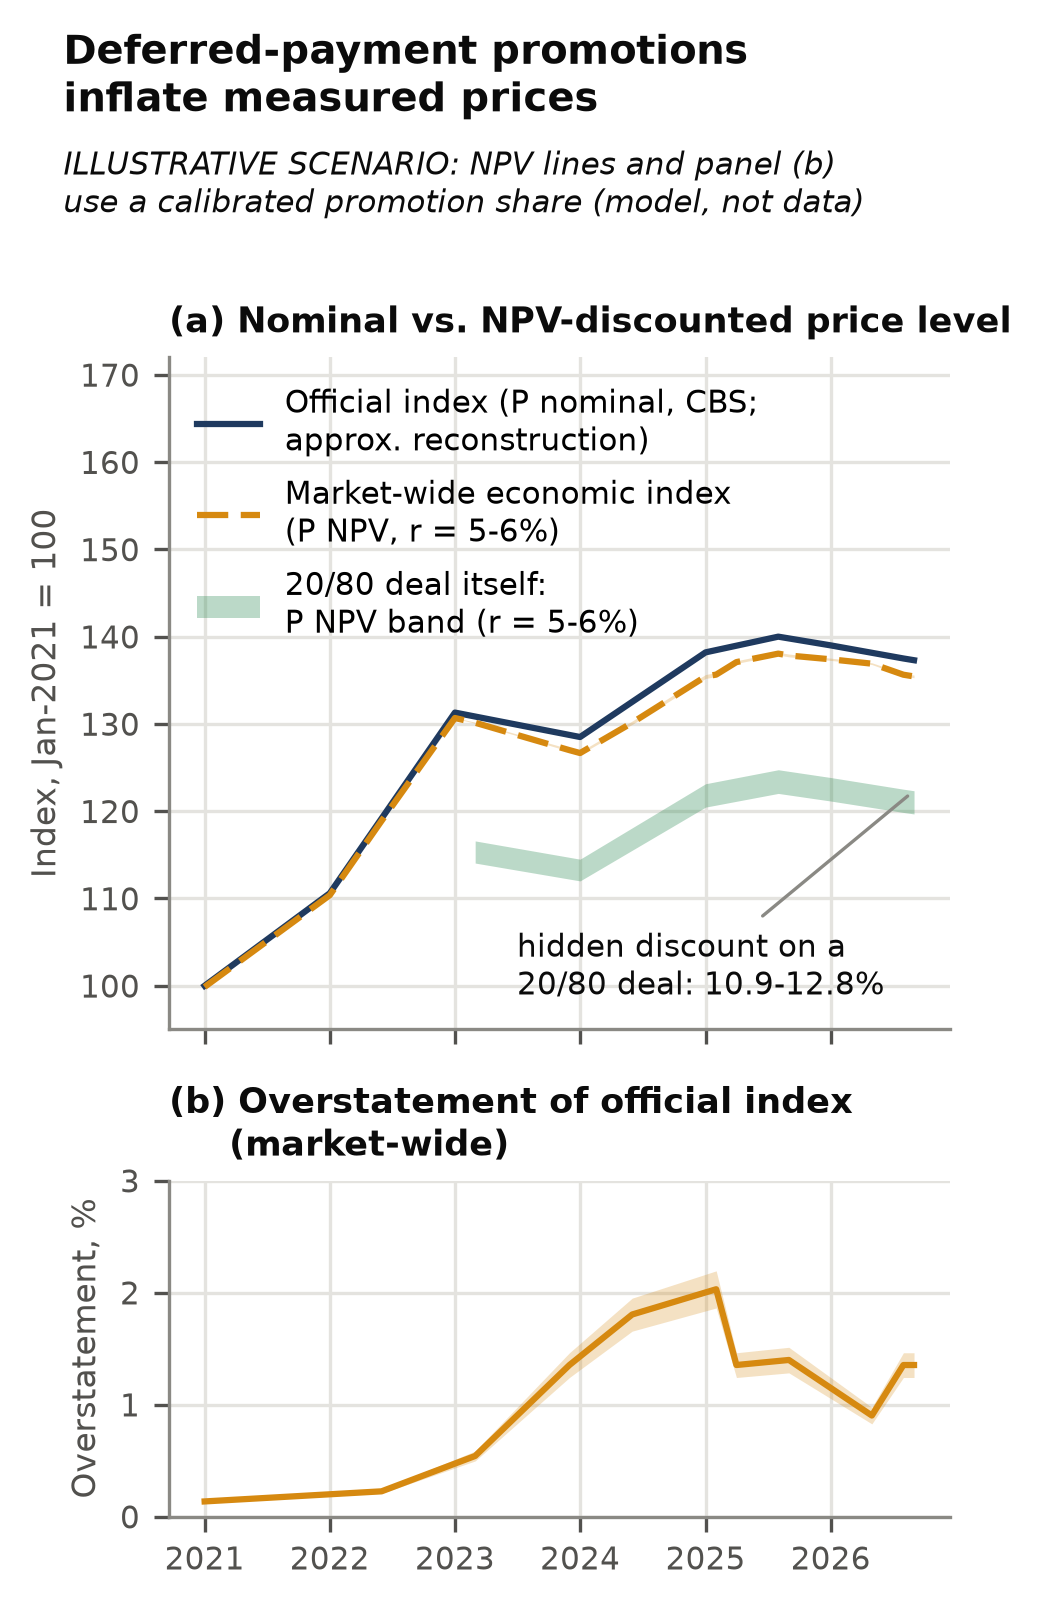
\includegraphics[width=0.55\textwidth]{figures/fig3_npv_price_discount_gap.png}
\caption[מדד המחירים הרשמי לעומת המחיר הכלכלי המהוון (\en{NPV})]{מדד מחירי הדירות הרשמי לעומת המחיר הכלכלי המהוון (\en{NPV}) בשיעור היוון של \en{5\%–6\%}. רמות המדד הרשמי הן שחזור משוער; קווי ה־\en{NPV} הם תרחיש להמחשה}
\label{fig:npv-gap}
\end{figure}

\paragraph{סימולציית מונטה קרלו של יחס ההחזר.}\label{subsec:ch5-mc} כדי לאמוד כמה קונים יחצו את ספי ה־\en{PTI} של הוראה \en{329} (סעיף~\ref{sec:ch3-baseline}) ביום המסירה, נדגמו \en{10,000} משקי בית. מחיר הדירה וההכנסה נדגמו מהתפלגות לוג־נורמלית דו־ממדית עם מתאם של \en{0.55}, שיעור המימון מהתפלגות \en{Beta(9,4)} שנקטעה ב־\pct{75}, תקופת ההלוואה \en{25} או \en{30} שנה, ונוסף זעזוע הכנסה אקראי עם סטיית תקן של \pct{5} בין החתימה למסירה. אותן דגימות שימשו לשלושה תרחישי ריבית משכנתה (\pct{4.00}, \pct{5.25} ו־\pct{6.50}).

\paragraph{רשת מבחני הקיצון ליזם ולבנק.}\label{subsec:ch5-stress} רשת מבחני הקיצון בוחנת פרויקט מייצג של \en{200} דירות (להמחשה), שמהן \pct{60} נמכרו מראש, בשני ממדים: ירידת מחירים של \en{0\%–20\%} ועיכוב במסירה של \en{0–24} חודשים (\en{81} תאים). ההכנסות מנורמלות ל־$R=1$, העלויות הן \en{0.83}, והאשראי הבנקאי $L$ הוא \pct{70} מהעלויות. כאשר הירידה במחיר עולה על \pct{5}, חלק מקוני המבצעים מבטלים, והדירות נמכרות מחדש בהנחה נוספת של \pct{5}. העיכוב מוסיף ארבעה רכיבי עלות: התייקרות בנייה, ריבית על האשראי, המשך סבסוד ריבית הבלון, ופיצוי לקונים לפי חוק המכר \cite{salelaw1974} (דמי שכירות מוכפלים, בהנחת \nis{7,500} לחודש). שני מדדי התוצאה הם:

\begin{align}
\mathrm{DSCR} &= \frac{\mathrm{Rev}(p,m) - C - O(m) + L}{L}, \label{eq:ch5-dscr}\\
\mathrm{Coverage} &= \frac{(1-p)\,R\,(1-h) - O(m)}{L + G}, \label{eq:ch5-coverage}
\end{align}

כאשר $O(m)$ עלויות העיכוב, $h$ קיצוץ ערך הבטוחה ו־$G$ ערבויות חוק המכר שהבנק נתן לקונים (\pct{30} מהתמורה ששולמה מראש). $\mathrm{DSCR}<1$ פירושו שהיזם אינו יכול לפרוע את האשראי מתזרים המסירה, ו־$\mathrm{Coverage}<100\%$ פירושו שהבטוחה אינה מכסה את חשיפת הבנק.

\paragraph{מודל שחיקת ההון העצמי רובד \en{1}.}\label{subsec:ch5-cet1} כשל של רוכש אינו כשל של בנק. הרוכש הנכשל מחזיר את הדירה ליזם, הדירה נמכרת מחדש בהנחה וכרית הביטחון של הפרויקט נשחקת; הבנק מפסיד רק כשהיא מתאפסת. הכרית נמדדת ב\term{כושר ספיגה}{Absorption Capacity}: הירידה המרבית במחירי המכירה שאינה גורמת לבנק הפסד \cite{boi_survey2025}. עבור שיעור כשל רוכשים $\delta$, ירידת מחיר $q$ ועיכוב $m$, השחיקה במונחי מחיר של המלאי שטרם נמכר היא:

\begin{equation}
x=q+\frac{\pi\varphi\,\delta\,[1-(1-q)(1-c)]+O(m)}{1-\pi}
\label{eq:ch5-erosion}
\end{equation}

כאשר $\pi=0.6$ שיעור המכירה המוקדמת, $\varphi=0.45$ חלק המבצעים ו־$c$ הנחת המכירה מחדש. חלק החשיפה הנכשל הוא $\zeta F(x)$, כאשר $F$ ההתפלגות המצטברת של כושר הספיגה לפי אשראי: \pct{8} מתחת ל־\pct{30} ו־\pct{33} מתחת ל־\pct{40} \cite{boi_survey2025}, ויתר הנקודות מדוחות לאומי והפועלים \cite{leumi_q3_2026,hapoalim_q3_2026}, שהגדרותיהם שונות (סעיף~\ref{sec:ch5-limitations}). ההפסד ושחיקת יחס ההון של בנק $b$ הם:

\begin{align}
N_b &= \max\{0,\; \ell\,(sD_b+gG_b)-sP_b\}, \quad \ell_A = \zeta F(x)\,[1-(1-q)(1-k)], \label{eq:ch5-loss}\\
\Delta\mathrm{CET1}_b &= \frac{N_b(1-t)}{\mathrm{RWA}_b}, \quad \ell_B = \zeta\,\frac{1-\pi}{\lambda}\int_0^{x}F(a)\,da, \label{eq:ch5-cet1}
\end{align}

כאשר $s$ חלק הדיור באשראי, $k$ עלות המימוש, $t$ שיעור המס ו־$\lambda=0.761$ החשיפה ליחידת הכנסה. גרסה $A$ שמרנית בירידות המחיר שנבחנו (לפרויקט שנכשל לא נותרה כרית, וירידת המחיר פועלת פעמיים); גרסה $B$ מודדת רק את עומק הגירעון וללא מכירת חירום. ערבות שמומשה נוספת לחשיפה מול הדירה שחזרה, ולכן אינה נספרת פעמיים. נכסי הסיכון קבועים ורווחי הבנק אינם מקוזזים. לפי תיעוד הצוות, הכלל נקבע לפני ההרצה: תנאי ה־\pct{10} מתקיים אם שתי הגרסאות עומדות בו בתרחיש (כשל \pct{25}, ירידה \pct{20}, \en{24} חודשים), אינו מתקיים אם שתיהן חורגות, ואם הן חלוקות התוצאה תלויה בשיטה ואינה מכריעה. הבחינה לפני מס; \mbox{\en{REQ-H3-01}} אינה קובעת בסיס מס, ולכן מדווחת גם התוצאה אחרי מס. חישוב ידני ללאומי ($A$) מחזיר את תוצאת הקוד (\en{194} נ״ב). טבלה~\ref{tab:ch5-banks} מציגה את נתוני הבנקים.

\begin{table}[!htb]
\centering
\caption[נתוני חמש הקבוצות הבנקאיות]{נתוני המודל לחמש הקבוצות הבנקאיות, \en{30.9.2026} (מיליארדי \en{₪}; יחסים באחוזים)}
\label{tab:ch5-banks}
\footnotesize
\begin{tabularx}{\tabmaxwidth}{>{\raggedleft\arraybackslash}p{3.1cm} C C C C C C C}
\toprule
\hd{קבוצה} & \hd{\en{CET1}} & \hd{מזערי} & \hd{\en{RWA}} & \hd{הון} & \hd{$D$} & \hd{$G$} & \hd{$P$} \\
\midrule
לאומי \cite{leumi_q3_2026} & \en{11.38} & \en{10.23} & \en{623.4} & \en{71.4} & \en{149.3} & \en{48.0} & \en{3.4} \\
הפועלים \cite{hapoalim_q3_2026} & \en{11.62} & \en{10.24} & \en{580.6} & \en{67.5} & \en{116.1} & \en{31.5} & \en{2.6} \\
מזרחי־טפחות \cite{mizrahi_q3_2026} & \en{10.10} & \en{9.60} & \en{368.1} & \en{36.7} & \en{54.4} & \en{18.3} & \en{0.7} \\
דיסקונט \cite{discount_q3_2026} & \en{10.32} & \en{9.21} & \en{347.1} & \en{35.1} & \en{56.5} & \en{17.5} & \en{1.3} \\
הבינלאומי \cite{fibi_q3_2026} & \en{10.28} & \en{9.24} & \en{143.3} & \en{14.5} & \en{24.5} & \en{3.0} & \en{0.5} \\
\bottomrule
\end{tabularx}

\smallskip
$D$ חובות בינוי ונדל״ן בישראל; $G$ ערבויות לרוכשי דירות (נומינלי, לפני ביטוח משנה); $P$ הפרשה להפסדי אשראי
\end{table}

\section{כיול הפרמטרים ומגבלות}
\label{sec:ch5-calibration}

טבלה~\ref{tab:ch5-calibration} מרכזת את הפרמטרים המכוילים; רק מרכיבי $s$ ושיעור המס הם נתונים ממקור.

\begin{table}[!htb]
\centering
\caption[פרמטרים מכוילים (להמחשה)]{פרמטרים מכוילים (להמחשה), ערכיהם והנימוק לבחירתם}
\label{tab:ch5-calibration}
\footnotesize
\begin{tabularx}{\tabmaxwidth}{>{\raggedleft\arraybackslash}p{4.0cm} >{\centering\arraybackslash}p{2.7cm} R}
\toprule
\hd{פרמטר} & \hd{ערך} & \hd{נימוק} \\
\midrule
שיעור היוון $r$ & \en{5\%–6\%} & פריים ועוד מרווח \\
דחיית תשלום $T$, חלק נדחה $d$ & \en{3} שנים, \en{0.8} & בנייה טיפוסית, \en{20/80} \\
משקל דירות חדשות $w_{\mathrm{new}}$ & \en{0.38} & סדר גודל של חלקן בעסקאות \\
שיעור מבצעים $s(t)$ & \en{3\%–45\%} & \pct{30} באוגוסט \en{2026} (חמישה אזורים, מסירה משנה ומעלה) \cite{mof_review_2026_08} \\
מחיר והכנסה חציוניים & \nis{2.4M}, \nis{26,000} & סדר גודל \\
ריביות משכנתה & \pct{4.0}, \pct{5.25}, \pct{6.5} & ריבית \pct{3.25} ועוד מרווחים \\
שולי רווח יזם, אשראי לעלות & \pct{17}, \pct{70} & ליווי סגור, סדר גודל \\
ריבית אשראי יזם & \pct{7.25} & פריים \pct{4.75} ועוד \pct{2.5} \\
קוני מבצעים במכירה מוקדמת & \pct{45} & שיעור המבצעים בשיאו \\
קיצוץ ערך בטוחה $h$ & \pct{10} & מכירה כפויה \\
חלק הדיור $s$ & \pct{40.9} & \en{150/367}: פרויקטים וקרקע למגורים \cite{boi_survey2025} \\
מימוש ערבויות $g$, העברה $\zeta$ & \en{1}, \en{1} & שמרני; נבחן \en{0–0.5}, \en{0.25–0.5} \\
עלויות $c$, $k$; מס $t$ & \pct{5}, \pct{5}; \pct{34.75} & להמחשה; סטטוטורי \cite{discount_q3_2026} \\
כשל רוכשים, ירידת מחיר & \en{15\%–25\%} & \en{PTI} מעל \pct{50} באיור~\ref{fig:pti-mc} (\en{16\%–27\%}); תרחיש \\
\bottomrule
\end{tabularx}
\end{table}

\label{sec:ch5-limitations}שלוש מגבלות עיקריות: (\en{1}) הפרויקט ברשת מייצג ואינו מדגם, ופיזור מאזני היזמים רחב יותר; (\en{2}) עוגני \en{2021–2023} במלאי ובעסקאות לא אומתו; (\en{3}) המודלים אינם כוללים השפעות חוזרות (ירידת מחירים, ביטולים, גידול במלאי וירידה נוספת), ולכן תוצאות הרשת עשויות להמעיט בסיכון. מודל ההון מאחד נתוני כושר ספיגה משני מועדים, מייחס אותם גם לקרקע ומחיל חלק דיור אחיד על כל הבנקים; הוא אינו מבחן קיצון רשמי. גם ההגדרות שונות: לאומי מודד את כושר הספיגה מול מחירי המלאי, והפועלים (\pct{53} מהאשראי בשלוש מהנקודות) מול שווי הנכס כגמור; המודל מחיל את הגדרת לאומי, והשנייה הופכת את התוצאה (סעיף~\ref{sec:ch6-cet1}).

% =====================================================================
% פרק 6 — עמידות המערכת מול ״קיר המסירות״ 2026–2027 ובחינת ההשערות
% RESEARCH_CORE_AGENT (Agent 2)
% =====================================================================
\chapter{עמידות המערכת מול ״קיר המסירות״}
\label{ch:delivery-wall}

\begin{managerbox}
ביום המסירה הרוכש צריך לקבל משכנתא, היזם צריך לגבות את יתרת התמורה כדי לפרוע את אשראי הליווי, והבנק צריך שהבטוחה תכסה את חשיפתו, כולל ערבויות חוק המכר. הפרק מאתר את ספי הכשל ומכריע בהשערות. למעקב: הריבית, המחירים והעיכובים.
\end{managerbox}

\section{צד הרוכשים: יחס ההחזר ביום המסירה}
\label{sec:ch6-buyers}\label{sec:ch6-facts}

רוכש שחוצה את תקרת ה־\pct{50} של הוראה \en{329} (סעיף~\ref{sec:ch3-baseline}) לא יקבל את מלוא המשכנתא, ויצטרך להשלים הון, למכור את הזכות או לבטל (סימולציה: איור~\ref{fig:pti-mc}). התוצאות הן תרחיש, לא תחזית (סעיף~\ref{sec:ch5-limitations}).

\begin{figure}[!htb]
\centering
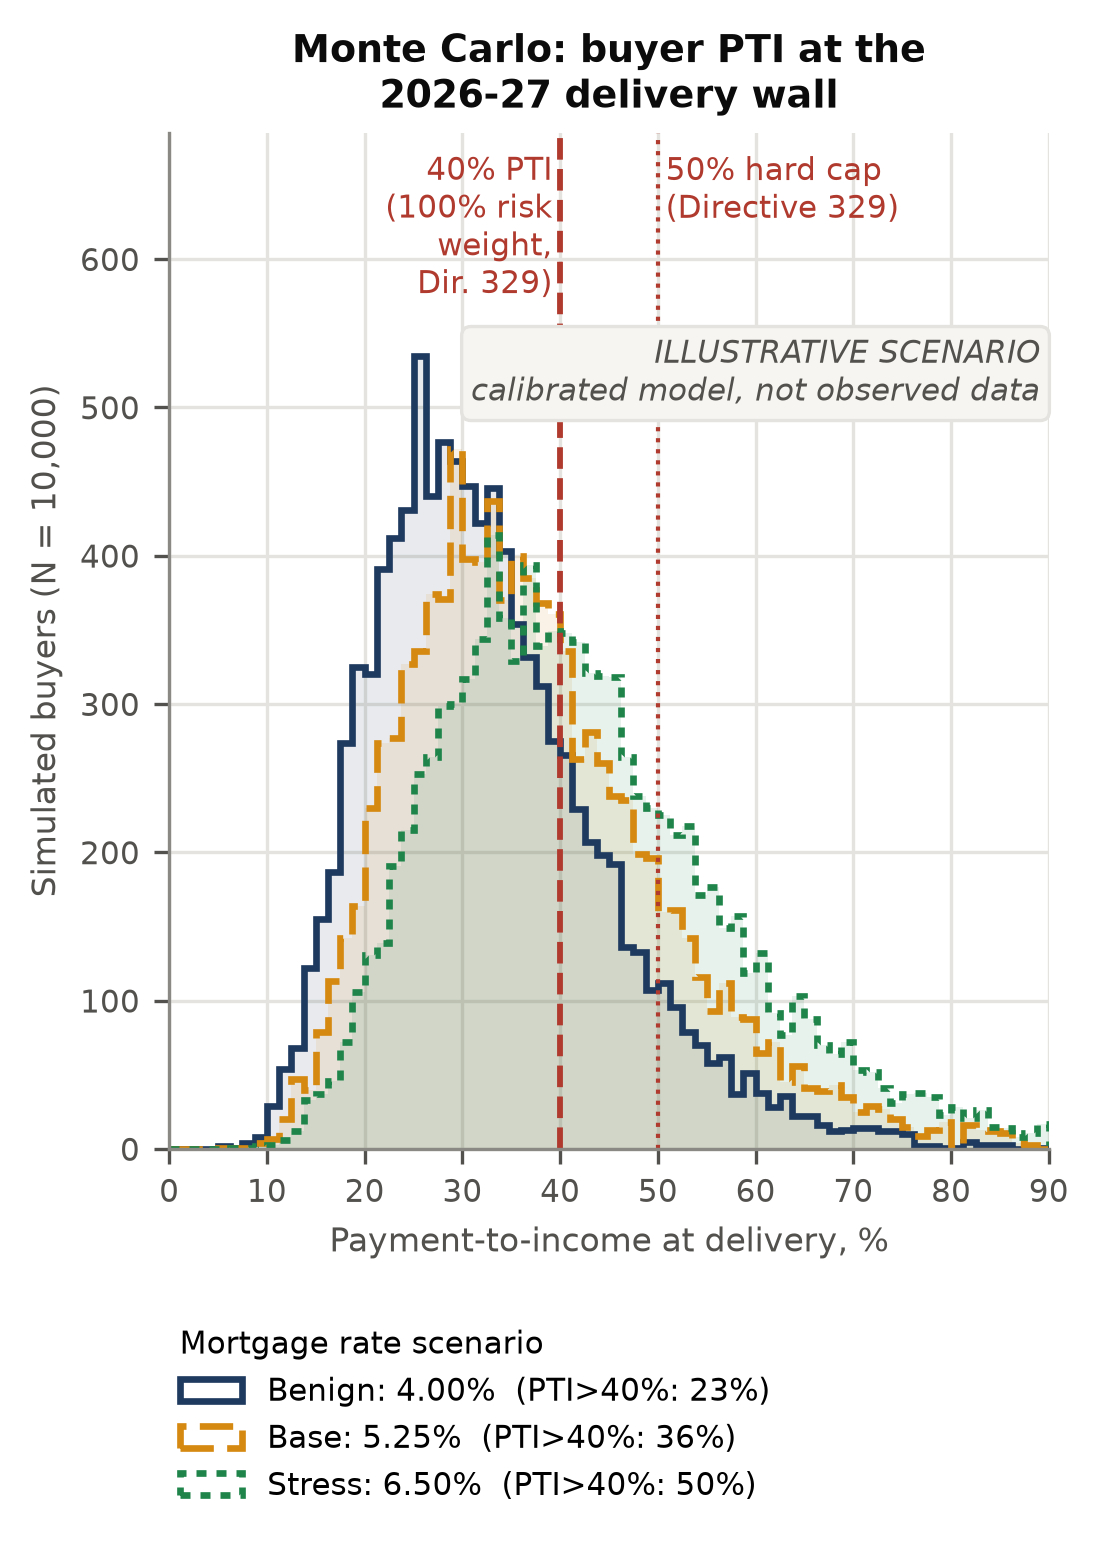
\includegraphics[width=0.62\textwidth]{figures/fig4_pti_monte_carlo.png}
\caption[יחס ההחזר ביום המסירה בשלושה תרחישי ריבית (תרחיש)]{התפלגות יחס ההחזר מההכנסה ביום המסירה (מונטה קרלו, \en{N=10,000}; תרחיש להמחשה)}
\label{fig:pti-mc}
\end{figure}

\label{tab:ch6-pti}בריביות \pct{4.00}, \pct{5.25} ו־\pct{6.50}, בהתאמה, החציון הוא \pct{30.9}, \pct{35.4} ו־\pct{40.2} (אחוזון \en{90}: \pct{48.2}, \pct{55.3} ו־\pct{62.7}); \pct{23.1}, \pct{36.1} ו־\pct{50.5} מהרוכשים חוצים את \pct{40}, ו־\pct{8.4}, \pct{16.0} ו־\pct{26.7} חוצים את \pct{50}. הריבית היא אפוא המשתנה הדומיננטי. סייגים: חציון המחיר וההכנסה הם הנחות, והרוכש אינו יכול להגדיל הון עצמי במודל.


\section{צד היזמים והבנקים: רשת מבחני הקיצון}
\label{sec:ch6-developers}

איור~\ref{fig:stress-grid} מציג את \term{יחס כיסוי שירות החוב}{DSCR} של היזם (משוואה~\ref{eq:ch5-dscr}) ואת כיסוי הבטוחות של הבנק (משוואה~\ref{eq:ch5-coverage}) בפרויקט המייצג.

\begin{figure}[!htb]
\centering
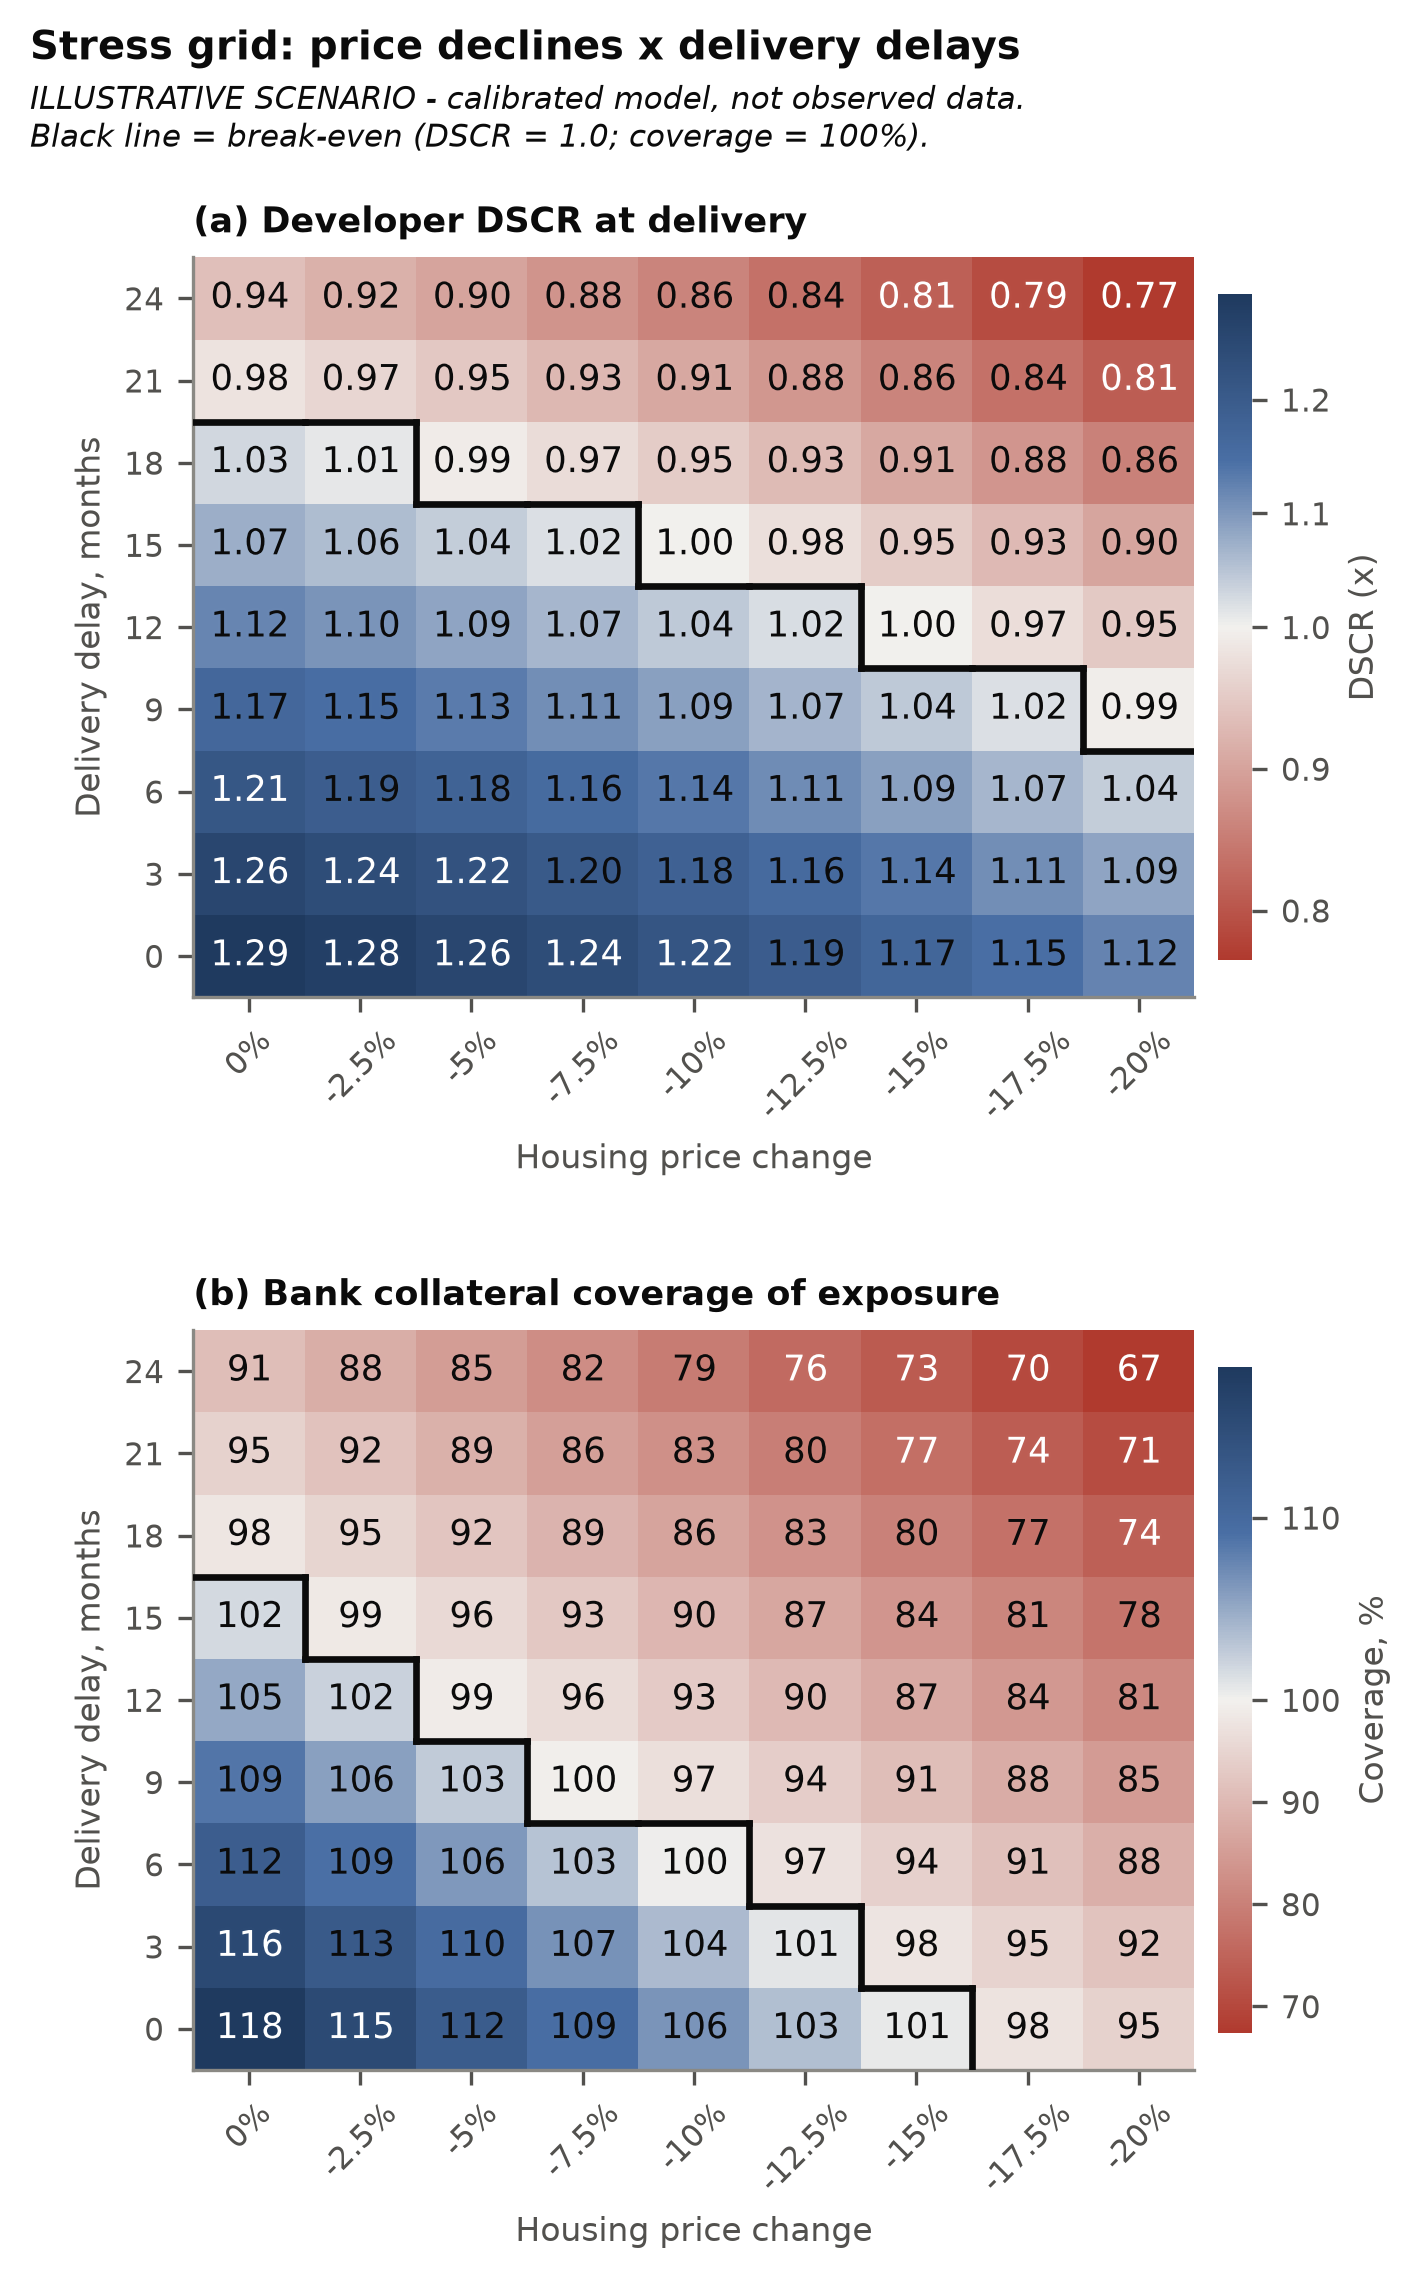
\includegraphics[width=0.85\textwidth]{figures/fig5_delivery_wall_resilience_heatmap.png}
\caption[רשת מבחני קיצון: \en{DSCR} וכיסוי הבטוחות (תרחיש)]{רשת מבחני קיצון לפרויקט מייצג: (\en{a}) \en{DSCR} של היזם; (\en{b}) כיסוי הבטוחות של הבנק כאחוז מחשיפתו. הקו השחור מסמן את נקודת האיזון. תרחיש מכויל להמחשה}
\label{fig:stress-grid}
\end{figure}

\textbf{היזם.} בתרחיש הבסיס ה־\en{DSCR} הוא \en{1.29}, ובתרחיש החמור ביותר ברשת (\pct{-20}, \en{24} חודשים) \en{0.77}. ב־\en{34} מתוך \en{81} תאים הוא נמוך מ־\en{1}; כבר בלחץ מתון (\pct{-10}, \en{12} חודשים) הוא רק \en{1.04}.

\textbf{הבנק.} הכיסוי יורד מ־\pct{118} בבסיס ל־\pct{67} בתרחיש החמור, וב־\en{57} מתוך \en{81} תאים הוא נמוך מ־\pct{100}. כשהיזם נכשל, ערבויות חוק המכר מגדילות את חשיפת הבנק כשהבטוחה נשחקת.

\textbf{רגישות.} עיכוב של שלושה חודשים שקול בקירוב לירידת מחירים של \pct{5} עבור ה־\en{DSCR} של היזם, ולירידה של \en{2.5\%–3\%} עבור כיסוי הבטוחות של הבנק.

\section{צד הבנקים: שחיקת ההון העצמי}
\label{sec:ch6-cet1}

לפי מודל שחיקת ההון (סעיף~\ref{subsec:ch5-cet1}), בתרחיש החמור שנקבע מראש (כשל רוכשים של \pct{25}, ירידת מחירים של \pct{20} ועיכוב של \en{24} חודשים) ההפסד לפני מס הוא \nis{48.0} מיליארד, \pct{21.3} מההון העצמי של המערכת, בגרסה $A$ השמרנית, ו־\nis{31.9} מיליארד, \pct{14.2}, בגרסה $B$ המבנית (אחרי מס: \pct{13.9} ו־\pct{9.2}). יחס \term{ההון העצמי רובד \en{1}}{CET1} המערכתי יורד מ־\pct{10.96} ל־\pct{9.44} ($A$, \en{152} נ״ב) או ל־\pct{9.96} ($B$, \en{101} נ״ב; איור~\ref{fig:cet1-erosion}).

\begin{figure}[!htb]
\centering
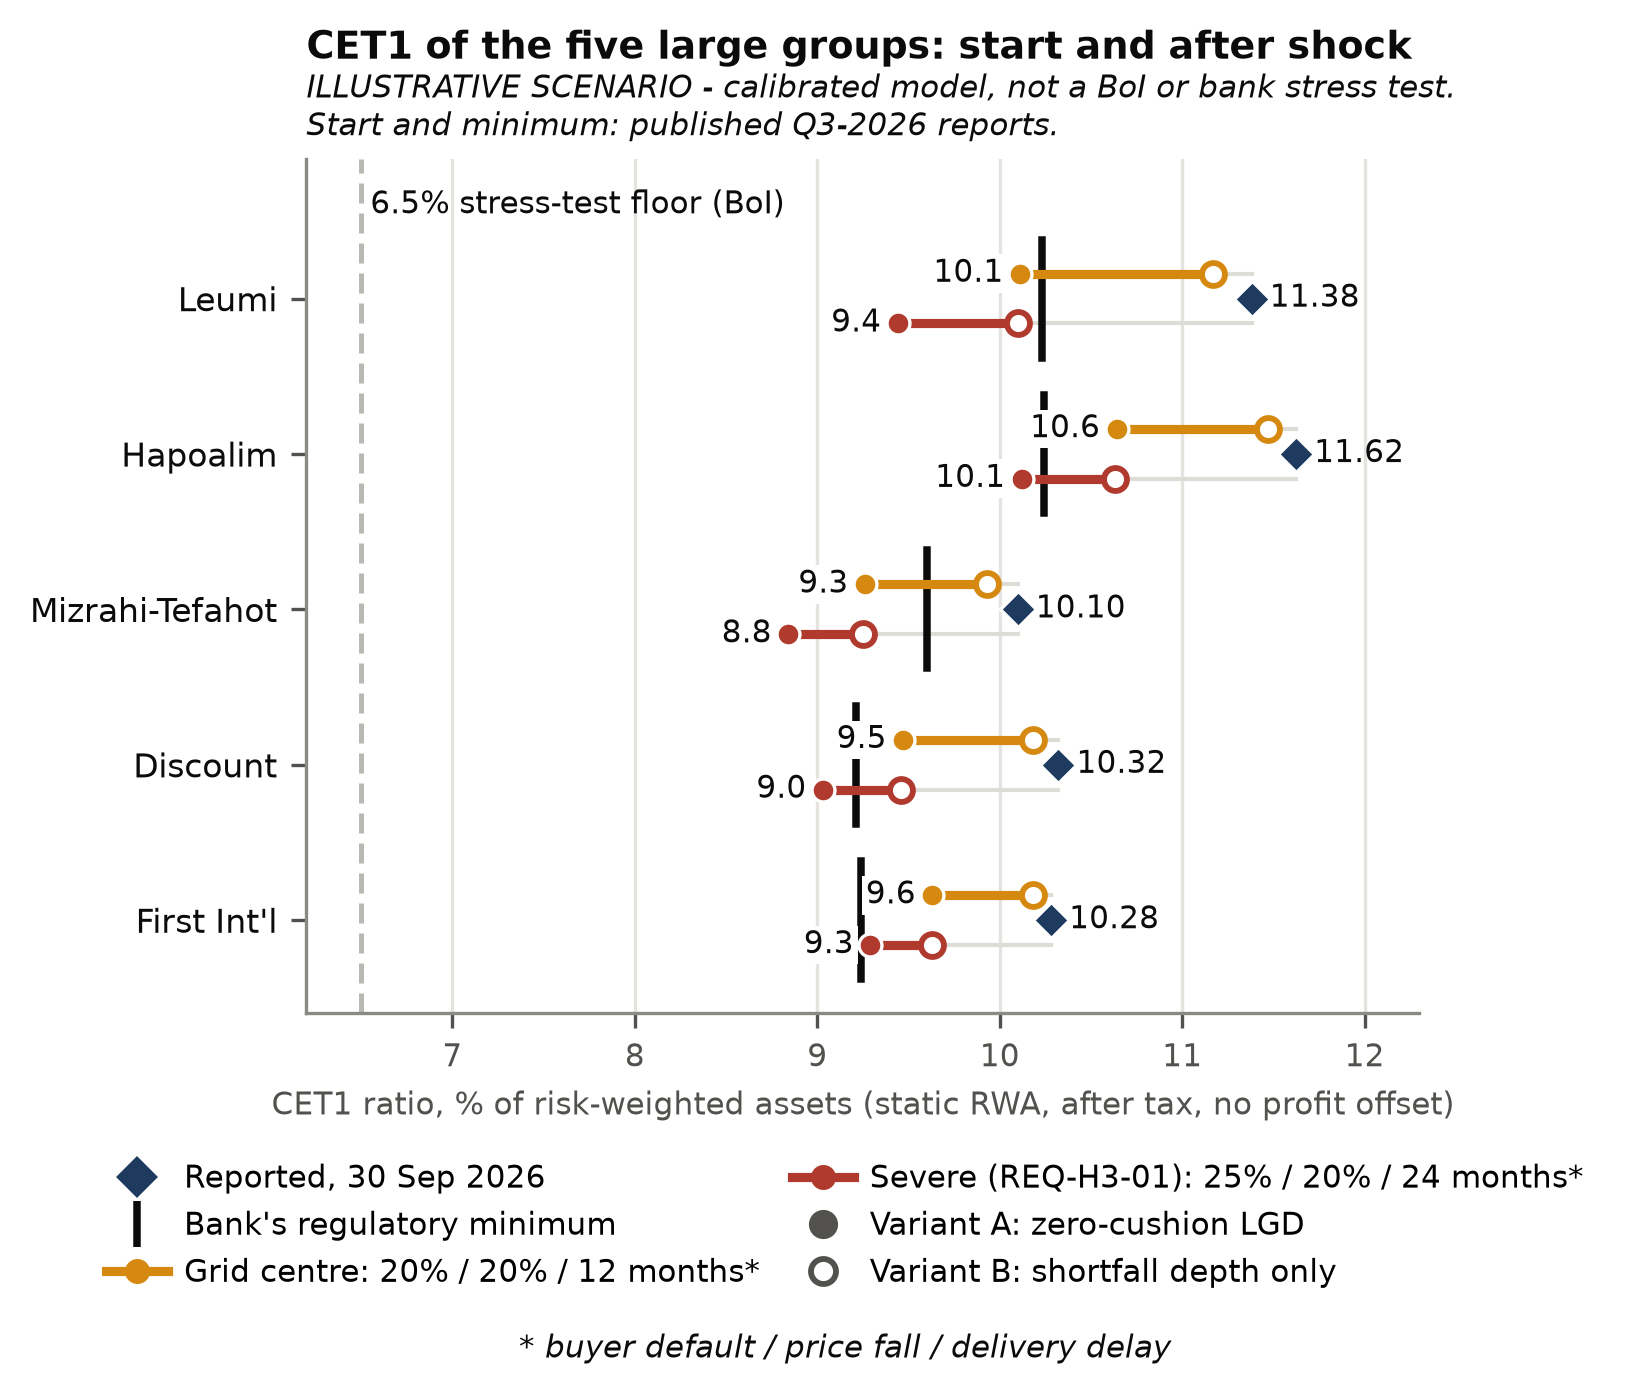
\includegraphics[width=0.85\textwidth]{figures/fig7_bank_cet1_erosion.png}
\caption[יחס \en{CET1} של הבנקים לפני הזעזוע ואחריו (תרחיש)]{יחס \en{CET1} לפני הזעזוע ואחריו מול המזערי (מלא: $A$; ריק: $B$; תרחיש, לא מבחן רשמי)}
\label{fig:cet1-erosion}
\end{figure}

\textbf{היחס המזערי (להמחשה).} בגרסה $A$ ארבע קבוצות יורדות אל מתחת ליחס המזערי (טבלה~\ref{tab:ch5-banks}): לאומי (\pct{9.44}), הפועלים (\pct{10.12}), מזרחי־טפחות (\pct{8.84}) ודיסקונט (\pct{9.03}); הבינלאומי נותר מעליו (\pct{9.29}). בגרסה $B$ רק לאומי (\pct{10.10}) ומזרחי־טפחות (\pct{9.25}). חריגה מיחס מזערי אינה חדלות פירעון: באף אחד מהתרחישים שנבחנו בפרמטרי הבסיס (עד כשל \pct{40}, ירידה \pct{40} ו־\en{24} חודשים) אין בנק היורד אל מתחת ל־\pct{6.5}, רצפת מבחני הקיצון \cite{boi_survey2024}; בגרסה $A$ (כשל \pct{25}, \en{24} חודשים) היא נחצית לראשונה בירידה של \pct{41.2}.

\textbf{עמידות הממצא.} כל \en{25} התאים בעיכוב של \en{24} חודשים חורגים מ־\pct{10} בשתי הגרסאות (טבלה~\ref{tab:ch6-grid}; שורות: כשל $\delta$, עמודות: ירידה $q$). ב־\en{12} חודשים טווח ההפסד הוא \en{7.5\%–19.9\%} ($A$) ו־\en{0.5\%–4.8\%} ($B$), ובמרכז הרשת \pct{14.0} ו־\pct{2.4}; ללא עיכוב הוא לכל היותר \pct{1.3} ($A$) ואפס ($B$). כשל רוכשים לבדו אינו יוצר הפסד בנקאי.

\begin{table}[!htb]
\centering
\caption[רשת \en{5×5}: הפסד בנקאי ב־\en{24} חודשים (תרחיש)]{הפסד בנקאי ב־\en{24} חודשים, אחוז מההון לפני מס (\en{A / B}; תרחיש; מודגש: ההכרעה)}
\label{tab:ch6-grid}
\footnotesize
\begin{tabularx}{\tabmaxwidth}{>{\centering\arraybackslash}p{1.9cm} C C C C C}
\toprule
\hd{$\delta$ / $q$} & \hd{\pct{15}} & \hd{\pct{17.5}} & \hd{\pct{20}} & \hd{\pct{22.5}} & \hd{\pct{25}} \\
\midrule
\pct{15} & \en{15.4 / 10.7} & \en{18.1 / 12.0} & \en{20.9 / 13.3} & \en{24.0 / 14.7} & \en{27.2 / 16.1} \\
\pct{17.5} & \en{15.5 / 10.9} & \en{18.2 / 12.2} & \en{21.0 / 13.5} & \en{24.1 / 14.9} & \en{27.4 / 16.4} \\
\pct{20} & \en{15.5 / 11.0} & \en{18.3 / 12.4} & \en{21.1 / 13.7} & \en{24.2 / 15.2} & \en{27.6 / 16.6} \\
\pct{22.5} & \en{15.6 / 11.2} & \en{18.3 / 12.5} & \en{21.2 / 13.9} & \en{24.4 / 15.4} & \en{27.7 / 16.9} \\
\pct{25} & \en{15.7 / 11.3} & \en{18.4 / 12.7} & \textbf{\en{21.3 / 14.2}} & \en{24.5 / 15.6} & \en{27.9 / 17.2} \\
\bottomrule
\end{tabularx}
\end{table}

\textbf{רגישות התרחיש החמור ($A$; $B$).} \emph{שתי הגרסאות מתחת ל־\pct{10}:} שיעור העברה $\zeta$ של \en{0.5} (\pct{9.9}; \pct{6.3}) או \en{0.25} (\pct{4.2}; \pct{2.4}), וכושר ספיגה על מלוא ערך הפרויקט, כהגדרת הפועלים (\pct{9.98}; \pct{0.6}). \emph{חלוקות:} אחרי מס (\pct{13.9}; \pct{9.2}) וללא מימוש ערבויות (\pct{11.8}; \pct{7.6}). \emph{שתיהן מעל \pct{10}:} מימוש \pct{50} מהערבויות (\pct{16.5}; \pct{10.9}), אשראי לפרויקטים בלבד (\pct{15.0}; \mbox{\pct{10.05}}), עלות מימוש של \pct{10} (\pct{25.1}; \pct{14.2}), כל חובות הענף, $s=1$ (\pct{38.3}; \pct{25.1}), וסיכון האשראי הכולל (\pct{49.1}; \pct{32.5}). מגבלות: \en{RWA} קבועים ואין קיזוז רווחים; במזרחי־טפחות סיכון הערבויות המדווח בענף הוא \nis{7.6} מיליארד, רובו בביטוח משנה (\nis{18.3} נומינלי במודל), ואשראי הליווי כ־\pct{59} מהאשראי המאזני לענף \cite{mizrahi_q3_2026}. מבחן הקיצון של בנק ישראל (\en{CET1} יורד ב־\en{1.5} נקודות אחוז, הפסד \pct{3.3} מהאשראי לענף) \cite{boi_survey2025} כולל רווחים ומאזן דינמי ואינו תיקוף.

\section{בחינת השערות המחקר}
\label{sec:ch6-hypotheses}

\begin{researchquestion}[השערה \en{H1}]
\textbf{\en{H1} — אשראי צל וקשיחות מחירים מלאכותית:} מבצעי המימון הקבלניים (\deal{20/80}, \deal{20/50/30}) והלוואות הבלון תפקדו כאשראי צל \enb{Shadow Credit} שעקף את מגבלות שיעור המימון (\en{LTV}) ויחס ההחזר מההכנסה (\en{PTI}) של בנק ישראל, ויצרו קשיחות מלאכותית של מחירי המחירון, תוך הסוואת ירידה ריאלית במחיר הכלכלי של הדירה במונחי ערך נוכחי נקי (\en{NPV}).
\end{researchquestion}

\textbf{קביעה: נתמכת חלקית.} סף \mbox{\en{REQ-H1-01}} (טבלה~\ref{tab:ch1-requirements}) מתקיים בתרחיש: ההנחה הגלומה במבצע \deal{20/80} היא \en{10.9\%–12.8\%}, מעל \pct{5} בכל שיעורי ההיוון. גם סף \mbox{\en{REQ-H1-02}}, פער חיובי מתמשך בין המדד הרשמי למדד המתוקן, מתקיים, אך הפער קטן: \pct{2.0} לכל היותר בשיאו ו־\pct{1.4} בספטמבר \en{2026} (איור~\ref{fig:npv-gap}), כי ההנחה מדוללת בעסקאות יד שנייה. מבחני ה־\en{LTV} וה־\en{PTI} נדחו (ולא בוטלו), פער העיתוי התארך \cite{boi2026_resloans}, והפיקוח הגביל את הלוואות הבלון המסובסדות \cite{boi_circular2816}. מנגד, מדד המחירים ירד ב־\pct{1.8} בשנה שעד אוגוסט \en{2026} \cite{toi_housing_2026_10}, כך שהקשיחות חלקית.

\begin{researchquestion}[השערה \en{H2}]
\textbf{\en{H2} — לחץ החזר בעת ״קיר המסירות״:} רמת ריבית המשכנתאות הגבוהה בתקופת ״קיר המסירות״ (\en{2026–2027}) תדחוף שיעור מהותי מרוכשי הדירות בתשלומים נדחים אל מעבר לסף יחס ההחזר של \pct{40} מההכנסה (\en{PTI}), שמעליו חל משקל סיכון מוגבר, ותוביל למצוקת מימון מחדש \enb{Refinancing Distress} ולביטולי עסקאות פוטנציאליים.
\end{researchquestion}

\textbf{קביעה: נתמכת בתרחיש, בכפוף לריבית.} סף \en{REQ-H2-01} דורש שבתרחיש הבסיס לפחות \pct{20} מהרוכשים יהיו מעל \pct{40}; השיעור הוא \pct{36.1}, וגם בתרחיש הנוח \pct{23.1}. סייגים: האיסור בהוראה \en{329} חל רק מעל \pct{50} \cite{boi_directive329}, והשיעור שחוצה סף זה נמוך יותר (\en{8\%–27\%}); ההפחתות מקטינות את סבירות הלחץ; ואין נתונים על הון הרוכשים, שבו תלויים הביטולים.

\begin{researchquestion}[השערה \en{H3}]
\textbf{\en{H3} — הסטת הסיכון המערכתי ליזמים:} בשל הבלמים המוסדיים — חוק המכר (דירות), מנגנון הליווי הבנקאי הסגור, מגבלות \en{LTV/PTI} נוקשות והלוואות בחבות אישית מלאה \enb{Full Recourse} — הסיכון המערכתי בישראל מתרכז במאזני היזמים ובמלאי הדירות הלא־מכורות (למעלה מ־\en{85,000} יחידות) ולא בחדלות פירעון של הבנקים, כפי שאירע בארה״ב ובספרד ב־\en{2008}.
\end{researchquestion}

\textbf{קביעה: אינה נתמכת לפי סף ההכרעה; הקביעה שברירית.} לסף \mbox{\en{REQ-H3-01}} שני תנאים. הראשון, \en{DSCR} נמוך מ־\en{1} בתרחיש החמור, מתקיים (\en{0.77}). השני, הפסד בנקאי של פחות מ־\pct{10} מההון העצמי של המערכת, אינו מתקיים: \pct{21.3} ($A$) ו־\pct{14.2} ($B$). הסף נבחן לפני מס, לפי הכלל; אחרי מס הגרסאות חלוקות (\pct{13.9} ו־\pct{9.2}), ולפי אותו כלל התוצאה אינה מכריעה. הרכיב התיאורי נתמך בחלקו: הסיכון הישיר מרוכז ביזמים ובמלאי (\en{85,080} דירות \cite{cbs_newdwellings_2026q3}, גידול של כ־\pct{40} באשראי לפרויקטים \cite{boi2026_recredit}), ושלושה ממנגנוני המשבר האמריקאי (איגוח נרחב, מינוף גבוה של משקי הבית והיעדר חבות אישית) אינם משוחזרים בישראל (פרק~\ref{ch:comparative}). אולם בזעזוע משולב וחמור הליווי וערבויות חוק המכר מעבירים לבנקים הפסד המוריד חלק מהם אל מתחת ליחס המזערי, אף שאין זו חדלות פירעון. בנק ישראל מעריך שמרווחי הביטחון בפרויקטים עדיין רחבים יחסית \cite{boi2026_recredit}, והקביעה תלויה בהנחות המודל (סעיף~\ref{sec:ch6-cet1}).

\begin{keyfinding}
\en{H1} נתמכת חלקית; \en{H2} נתמכת בתרחיש הבסיס; \en{H3} אינה נתמכת לפי הסף שנקבע מראש: ההפסד הבנקאי בתרחיש החמור (\en{14.2\%–21.3\%} מההון) חורג מ־\pct{10} לפני מס; אחרי מס התוצאה אינה מכריעה. הממצא שברירי ואינו מעיד על חדלות פירעון.
\end{keyfinding}


% =====================================================================
% פרק 7 — תוכנית עבודה, ניהול סיכונים וסיכום
% RESEARCH_CORE_AGENT (Agent 2)
% =====================================================================
\chapter{ניהול סיכונים, תוכנית עבודה וסיכום}
\label{ch:risks-gantt}

\begin{managerbox}
ממצאי פרק~\ref{ch:delivery-wall} מבוססים על מודלים מכוילים, ואת חלקם יש לתקף מול נתוני המסירות של \en{2026–2027}. פרק זה מתאר מה ייעשה בשלב המימוש, מי אחראי, מתי ומה עלול להשתבש, ונחתם בסיכום ובשלוש פעולות מיידיות.
\end{managerbox}

\section{פירוק העבודה, אחריות ולוח זמנים}
\label{sec:ch7-wbs}

\term{מבנה פירוק העבודה}{WBS} מחלק את שלב המימוש לחמש חבילות, שנגזרו מהפערים שזוהו: נתוני מסירות וביטולים ברמת הפרויקט, כיול המודלים לנתונים אלה, וחידוד אומדן ההפסד הבנקאי \enb{REQ-H3-01} בנתוני פרויקטים במקום בנתונים מצרפיים. טבלה~\ref{tab:ch7-wbs} מציגה לכל חבילה תוצר ו\term{מטריצת אחריות}{RACI}: מבצע (\en{R}), יועץ (\en{C}), מאשר (\en{A}). הצוות: שקד ניניו וגיא קובלרצ׳יק; מנחה: ד״ר יורם סגל.

\begin{table}[!htb]
\centering
\caption[חבילות העבודה ומטריצת האחריות]{חבילות העבודה, התוצרים ומטריצת האחריות (\en{RACI})}
\label{tab:ch7-wbs}
\small
\begin{tabularx}{\tabmaxwidth}{>{\centering\arraybackslash}p{1.2cm} R >{\centering\arraybackslash}p{0.9cm} >{\centering\arraybackslash}p{1.5cm} >{\centering\arraybackslash}p{0.8cm}}
\toprule
\hd{מזהה} & \hd{חבילה, משימות ותוצר} & \hd{ניניו} & \hd{קובלרצ׳יק} & \hd{סגל} \\
\midrule
\en{WP 1.0} & ספרות ומיפוי מבצעים ודוחות יזמים. \textbf{תוצר:} סקירה מעודכנת, מאגר מבצעים & \en{R} & \en{C} & \en{A} \\
\en{WP 2.0} & נתונים מהלמ״ס, בנק ישראל ורשות המסים, ואימותם. \textbf{תוצר:} מאגר מאומת & \en{C} & \en{R} & \en{A} \\
\en{WP 3.0} & כיול לנתונים; ראיונות עם בנקאי, שמאי ויזם. \textbf{תוצר:} מודלים מתוקפים & \en{C} & \en{R} & \en{A} \\
\en{WP 4.0} & תרחישים ומודל ההון בנתוני פרויקט; בחינת \en{H1–H3}. \textbf{תוצר:} פרק תוצאות & \en{R} & \en{C} & \en{A} \\
\en{WP 5.0} & כתיבה והגנה. \textbf{תוצר:} דוח ומצגת & \en{R} & \en{C} & \en{A} \\
\bottomrule
\end{tabularx}
\end{table}

\label{sec:ch7-gantt}לוח הזמנים מתפרס על \en{14} שבועות (איור~\ref{fig:ch7-gantt}). \term{הנתיב הקריטי}{Critical Path} עובר בסקירה, בנתונים, בכיול, בתרחישים (ובהם אומדן ההפסד המעודכן), בבחינת ההשערות ובכתיבה. אין בו מרווח; מרווח יש רק ב־\en{TSK-1.2} וב־\en{TSK-3.2}. נקבעו שתי אבני דרך לבקרה: \en{M-A} בסוף שבוע \en{7} (נתונים מאומתים ומודלים מכוילים) ו־\en{M-B} בסוף שבוע \en{11} (בחינת ההשערות הושלמה).

\begin{figure}[!htb]
\centering
\begin{english}
\begin{tikzpicture}[x=0.5cm, y=0.52cm, font=\footnotesize]
  % weeks run right -> left (Hebrew orientation); task labels on the right
  \foreach \w in {2,4,...,14}{ \fill[brandPale] (-\w+1,0.2) rectangle (-\w,-7.8); }
  \foreach \w in {1,...,14}{ \node[font=\scriptsize\bfseries, text=brandNavy] at (-\w+0.5,0.6) {\w}; }
  \foreach \w in {0,...,14}{ \draw[gray!35] (-\w,0.2) -- (-\w,-7.8); }
  \draw[brandNavy, line width=0.8pt] (-14,0.2) -- (13.8,0.2);
  \draw[brandNavy, line width=0.8pt] (-14,-7.8) -- (13.8,-7.8);
  \node[font=\scriptsize\bfseries, text=brandNavy, anchor=east] at (13.7,0.6) {\he{משימה}};
  \node[font=\scriptsize\bfseries, text=brandNavy] at (1.9,0.6) {\he{קודמות}};
  \node[font=\scriptsize\bfseries, text=brandNavy] at (-7,1.2) {\he{שבוע}};
  % ---- tasks: row / start week / length / code / label / critical ----
  \foreach \r/\s/\l/\code/\lab/\crit/\pre in {
     1/1/2/TSK-1.1/{סקירת ספרות}/1/{--},
     2/1/4/TSK-1.2/{מיפוי מבצעים}/0/{--},
     3/3/3/TSK-2.1/{איסוף ואימות נתונים}/1/{1.1},
     4/6/2/TSK-3.1/{כיול מודלים}/1/{2.1},
     5/5/4/TSK-3.2/{ראיונות מומחים}/0/{1.2},
     6/8/2/TSK-4.1/{תרחישים ורגישות}/1/{3.1},
     7/10/2/TSK-4.2/{בחינת השערות}/1/{4.1, 3.2},
     8/12/3/TSK-5.1/{כתיבה והגנה}/1/{4.2}}{
    \node[anchor=east] at (13.7,-\r+0.6) {\he{\lab}\ \ \texttt{\code}};
    \node at (1.9,-\r+0.6) {\pre};
    \ifnum\crit=1
      \fill[brandRed!85, rounded corners=1pt] (-\s+1,-\r+0.82) rectangle (-\s-\l+1,-\r+0.38);
    \else
      \fill[brandSteel, rounded corners=1pt] (-\s+1,-\r+0.82) rectangle (-\s-\l+1,-\r+0.38);
    \fi
  }
  % ---- milestones (end of week 7, end of week 11) ----
  \foreach \t/\tag in {7/M-A, 11/M-B}{
    \draw[brandAmber, dashed, line width=0.9pt] (-\t,0.2) -- (-\t,-7.8);
    \node[diamond, fill=brandAmber, draw=black!60, inner sep=2pt] at (-\t,-8.15) {};
    \node[font=\scriptsize\bfseries, anchor=north] at (-\t,-8.35) {\tag};
  }
  % ---- legend ----
  \begin{scope}[shift={(0,-9.5)}]
    \fill[brandRed!85] (8.8,0.15) rectangle (8.0,-0.15);
    \node[anchor=east] at (7.8,0) {\he{נתיב קריטי}};
    \fill[brandSteel] (3.6,0.15) rectangle (2.8,-0.15);
    \node[anchor=east] at (2.6,0) {\he{משימה עם מרווח}};
    \node[diamond, fill=brandAmber, draw=black!60, inner sep=2pt] at (-4.0,0) {};
    \node[anchor=east] at (-4.5,0) {\he{אבן דרך}};
  \end{scope}
\end{tikzpicture}
\end{english}
\caption[תרשים גאנט לשלב המימוש]{תרשים גאנט לשלב המימוש (\en{14} שבועות): משימות, משימות קודמות, נתיב קריטי ואבני דרך}
\label{fig:ch7-gantt}
\end{figure}

\section{ניתוח סיכונים ותוכנית הפחתה}
\label{sec:ch7-risks}

הסיכונים כאן הם של פרויקט המחקר, ולא של שוק הדיור. כל סיכון דורג לפי הסתברות $P$ והשפעה $I$ בסולם \en{1–5}, וציונו $R = P \times I$; ציון של \en{12} ומעלה מוגדר קריטי (טבלה~\ref{tab:ch7-risks} ואיור~\ref{fig:ch7-riskmatrix}).

\begin{table}[!htb]
\centering
\caption{זיהוי סיכוני המחקר וכימותם}
\label{tab:ch7-risks}
\small
\begin{tabularx}{\tabmaxwidth}{>{\centering\arraybackslash}p{2.4cm} R >{\centering\arraybackslash}p{0.6cm} >{\centering\arraybackslash}p{0.6cm} >{\centering\arraybackslash}p{0.7cm}}
\toprule
\hd{מזהה} & \hd{תרחיש הכשל} & \hd{\en{P}} & \hd{\en{I}} & \hd{\en{R}} \\
\midrule
\mbox{\en{RSK-DAT-01}} & נתוני מסירות וביטולים ברמת הפרויקט אינם מפורסמים או מתעכבים & \en{4} & \en{4} & \textbf{\en{16}} \\
\mbox{\en{RSK-MOD-02}} & הפרמטרים המכוילים אינם מייצגים את האוכלוסייה בפועל & \en{3} & \en{4} & \textbf{\en{12}} \\
\mbox{\en{RSK-SRC-03}} & נתון מרכזי זמין רק ממקור משני ואינו ניתן לאימות מול המפרסם & \en{3} & \en{4} & \textbf{\en{12}} \\
\mbox{\en{RSK-SCH-04}} & הנתיב הקריטי ללא מרווח; עיכוב במשימה אחת מעכב את ההגשה & \en{3} & \en{3} & \en{9} \\
\mbox{\en{RSK-SCP-05}} & התרחבות ההיקף, למשל לאשראי חוץ־בנקאי או לנדל״ן מסחרי & \en{3} & \en{3} & \en{9} \\
\mbox{\en{RSK-ENV-06}} & שינוי בריבית או ברגולציה (כגון סיום הוראת השעה) משנה את בסיס התרחיש & \en{4} & \en{2} & \en{8} \\
\bottomrule
\end{tabularx}
\end{table}

\begin{figure}[!htb]
\centering
\begin{english}
\begin{tikzpicture}[x=2.25cm, y=0.84cm, font=\footnotesize]
  % 5x5 matrix: x = impact I, y = probability P, score R = P*I; R >= 12 critical
  \foreach \p in {1,...,5}{ \foreach \i in {1,...,5}{
    \pgfmathtruncatemacro{\s}{\p*\i}
    \ifnum\s>11 \def\cc{brandRed!60}\else\ifnum\s>4 \def\cc{brandAmber!45}\else \def\cc{brandGreen!35}\fi\fi
    \fill[\cc, draw=white, line width=1.2pt] (\i-1,\p-1) rectangle (\i,\p);
    \node[anchor=north west, font=\scriptsize, inner sep=1.5pt, text=black!75] at (\i-1,\p) {\s};
  }}
  \foreach \i in {1,...,5}{ \node[anchor=north] at (\i-0.5,-0.05) {\i}; }
  \foreach \p in {1,...,5}{ \node[anchor=east] at (-0.03,\p-0.5) {\p}; }
  \node[anchor=north] at (2.5,-0.6) {\he{השפעה} ($I$)};
  \node[rotate=90, anchor=south] at (-0.22,2.5) {\he{הסתברות} ($P$)};
  \begin{scope}[every node/.style={font=\footnotesize\bfseries, align=center, inner sep=0pt}]
    \node at (3.6,3.5) {DAT-01};
    \node at (3.6,2.5) {MOD-02\\[-3pt]SRC-03};
    \node at (2.6,2.5) {SCH-04\\[-3pt]SCP-05};
    \node at (1.6,3.5) {ENV-06};
  \end{scope}
  \begin{scope}[shift={(5.12,0)}]
    \foreach \y/\c/\lab in {3.6/brandRed!60/{קריטי: \en{12–25}}, 2.5/brandAmber!45/{בינוני: \en{5–10}}, 1.4/brandGreen!35/{נמוך: \en{1–4}}}{
      \fill[\c] (0,\y-0.25) rectangle (0.2,\y+0.25);
      \node[anchor=west] at (0.25,\y) {\he{\lab}};
    }
  \end{scope}
\end{tikzpicture}
\end{english}
\caption[מטריצת הסיכונים \en{5×5}]{מטריצת הסיכונים \en{5×5}: המספר בכל תא הוא $R$; המזהים לפי טבלה~\ref{tab:ch7-risks} (ללא הקידומת \en{RSK})}
\label{fig:ch7-riskmatrix}
\end{figure}

\begin{table}[!htb]
\centering
\caption[פעולות מנע ותוכניות מגירה]{פעולות מנע, תוכניות מגירה וציון שיורי לסיכונים הקריטיים}
\label{tab:ch7-mitigation}
\small
\begin{tabularx}{\tabmaxwidth}{>{\centering\arraybackslash}p{2.4cm} R R >{\centering\arraybackslash}p{1.3cm}}
\toprule
\hd{מזהה} & \hd{פעולת מנע} & \hd{תוכנית מגירה} & \hd{שיורי} \\
\midrule
\mbox{\en{RSK-DAT-01}} & פנייה בשבוע \en{1} לפיקוח על הבנקים ולהלמ״ס; דוחות יזמים ציבוריים & אומדן מנתוני האשראי ומדוחות היזמים & \en{8} (\en{2×4}) \\
\mbox{\en{RSK-MOD-02}} & תיקוף בראיונות \enb{TSK-3.2}; הרחבת הרגישות & הצגת התוצאות כטווח ולא כערך נקודתי & \en{6} (\en{2×3}) \\
\mbox{\en{RSK-SRC-03}} & איתור הפרסום הראשי ושימוש בו בלבד & השמטה, או הצגה כמקור משני & \en{4} (\en{1×4}) \\
\bottomrule
\end{tabularx}
\end{table}

\newpage
לשלושת הסיכונים הקריטיים נקבעו פעולת מנע, תוכנית מגירה וציון שיורי (טבלה~\ref{tab:ch7-mitigation}); שלושת האחרים נמצאים במעקב.
\newpage
\section{סיכום: מוכנים לשלב המימוש}
\label{sec:ch7-summary}

\paragraph{עיקרי הממצאים.}
\begin{itemize}
  \item \textbf{מנגנונים}: שלושה ממנגנוני הכשל של \en{2008} משוחזרים בישראל: דחיית מבחן היכולת, זעזוע תשלום מרוכז ובנייה לפני מכירה. שלושה אינם משוחזרים: מינוף מצרפי גבוה של משקי הבית, איגוח נרחב והיעדר חבות אישית. הדמיון לספרד גדול מהדמיון לארה״ב (פרק~\ref{ch:comparative}).
  \item \textbf{\en{H1} נתמכת חלקית} ו־\textbf{\en{H2} נתמכת בתרחיש הבסיס}: כ־\pct{36} מהרוכשים במבצעים חוצים יחס החזר של \pct{40} ביום המסירה, וכ־\pct{16} חוצים את \pct{50} (סעיף~\ref{sec:ch6-buyers}).
  \item \textbf{\en{H3} אינה נתמכת לפי הסף שנקבע מראש}: בתרחיש החמור ה־\en{DSCR} של היזם יורד ל־\en{0.77}, אך ההפסד הבנקאי הוא \en{14.2\%–21.3\%} מההון העצמי לפני מס, מעל \pct{10}. הממצא שברירי: אחרי מס הגרסאות חלוקות (\pct{13.9} ו־\pct{9.2}) והתוצאה אינה מכריעה, ובשיעור העברה של \en{0.5} שתיהן מתחת ל־\pct{10}. כשל רוכשים לבדו אינו יוצר הפסד בנקאי, ובאף אחד מהתרחישים שנבחנו בפרמטרי הבסיס (עד \en{40\%/40\%/24}) אין בנק היורד אל מתחת ל־\pct{6.5} (סעיף~\ref{sec:ch6-cet1}).
\end{itemize}

\paragraph{מוכנות.} המודלים, ובהם מודל ההון, בנויים ומשחזרים את תוצאותיהם. החסר העיקרי הוא נתונים ברמת הפרויקט, שיחליפו את ההנחות שבהן תלויה הקביעה על \en{H3} (\mbox{\en{RSK-DAT-01}}). הציון השיורי של כל הסיכונים הקריטיים נמוך מ־\en{12}, ולכן המחקר מוכן לשלב המימוש.

\begin{keybox}[\en{3} פעולות מיידיות להמשך המחקר והיישום]
\textbf{(\en{1}) בקשת נתונים} (קובלרצ׳יק, שבוע \en{1}): מסירות, ביטולים וכושר ספיגה ברמת הפרויקט, מהפיקוח על הבנקים ומהלמ״ס. \textbf{תוצר:} בקשה מוגשת ורשימת שדות.\par
\textbf{(\en{2}) תיאום ראיונות} (קובלרצ׳יק, שבועות \en{1–2}): בנקאי מלווה, שמאי ויזם, לתיקוף שיעור ההעברה וכושר הספיגה. \textbf{תוצר:} שלושה מועדים ושאלון פרמטרים.\par
\textbf{(\en{3}) פגישת התנעה} (ניניו, שבוע \en{1}): אישור המנחה לתוכנית העבודה, לאבני הדרך ולבחינה החוזרת של \en{H3} בסף \pct{10} ללא שינוי. \textbf{תוצר:} פרוטוקול מאושר.
\end{keybox}


% ---------------- References (IEEE, biber) ----------------
\backmatter
\chapter{מקורות}                 % Hebrew RTL heading, in TOC, header "מקורות"
\begin{english}                 % entries are English -> LTR, IEEE numbering
\printbibliography[heading=none]
\end{english}

\end{document}
